\PassOptionsToPackage{dvipsnames}{xcolor}
\documentclass[10pt,externalviewer]{beamer}

\usepackage[dvipsnames]{xcolor}
\usepackage{amssymb}
\usepackage{rotating}
\usepackage{amsmath}
\usepackage{hyperref}
\usepackage{bookmark}
\usepackage{bigints}
\usepackage{graphics}
\usepackage{natbib}
\usepackage{relsize}
\usepackage{caption}
\usepackage{subcaption}
\usepackage{framed}
\usepackage{tikz}
\usepackage{lipsum}
\usepackage[italian]{babel}
\usepackage[utf8]{inputenc}
\usepackage[T1]{fontenc}
\usepackage[mode=math]{siunitx}
\usepackage[absolute,overlay]{textpos}
\usepackage{pdfcolparallel}
\usepackage[most]{tcolorbox}
\usepackage{physics}
\usetikzlibrary{decorations.pathreplacing}
\tcbuselibrary{fitting}

\tcbset{
  pythoncode/.style={
    listing only,
    listing options={language=Python, basicstyle=\ttfamily\small},
    enhanced,
    colback=gray!10,
    colframe=BrickRed,
    arc=2mm,
    boxrule=0.5pt,
    left=4pt,right=4pt,top=4pt,bottom=4pt,
  }
}

\renewcommand{\arraystretch}{2}

\makeatletter
\newcommand\xleftrightarrow[2][]{
  \ext@arrow 9999{\longleftrightarrowfill@}{#1}{#2}}
\newcommand\longleftrightarrowfill@{
  \arrowfill@\leftarrow\relbar\rightarrow}
\makeatother

\definecolor{PDred}{HTML}{9B0014}

\mode<presentation>
{
  \usetheme{Warsaw}
 %\usetheme{Madrid}
 %\usetheme{Montpellier}
 %\usetheme{Marburg} 
  \usecolortheme[named=PDred]{structure}
  \setbeamercolor{alerted text}{fg=PDred}
  \setbeamercovered{transparent}
  \setbeamertemplate{section in toc}[ball unnumbered]
  \usefonttheme[]{serif}
  \setbeamerfont{author}
  {size=\scriptsize,parent=structure}
  \setbeamerfont{date}
  {parent=structure}
  \setbeamerfont{title}
  {size=\Large,parent=structure}
  \setbeamerfont{sectiontitle}
  {size=\Large,parent=structure}
  \setbeamerfont{short title}
  {size=\tiny}
}

%\setbeamertemplate{footline}{\hfill\insertframenumber/\inserttotalframenumber} 

\expandafter\def\expandafter\insertshorttitle\expandafter{%
  \insertframenumber\,/\,\inserttotalframenumber}

\newcommand{\backupbegin}{
   \newcounter{framenumberappendix}
   \setcounter{framenumberappendix}{\value{framenumber}}
}
\newcommand{\backupend}{
   \addtocounter{framenumberappendix}{-\value{framenumber}}
   \addtocounter{framenumber}{\value{framenumberappendix}} 
}

\newcommand{\refer}[1]{%
   \begin{flushright}
      {\alert{\tiny #1}}
   \end{flushright}}
  
\newcommand{\lrefer}[1]{%
   \begin{flushleft}
      {\alert{\tiny #1}}
   \end{flushleft}}
  
\newcommand{\param}[1]{%
   \begin{flushright}
      {\small #1}
   \end{flushright}
   \vspace{-1.5\baselineskip}
}

%\newcommand{\sech}{\mathop{\rm sech}\nolimits}
\newcommand{\sgn}{\mathop{\rm sgn}\nolimits}
\newcommand{\etal}{{\em et al.}}


\title{Simulation and Analysis of 1D Wave Propagation under Various Physical Models}

\author[Dario Liotta]{\large{\textbf{Dario Liotta}}}

\institute[Physics of Data (UniPD)]{
\begin{minipage}[c]{3.4truecm}

\includegraphics[width=\textwidth]{logo-unipd}
\end{minipage}
\begin{minipage}[c]{2truecm}
   \begin{flushleft}
   \end{flushleft}
\end{minipage}
\begin{minipage}[c]{4.2truecm}

\includegraphics[width=\textwidth]{logo-dfa}
\end{minipage}}

\date{September 6th 2025 \\ Course of \textbf{Quantum Information and Computing} \\ Academic Year 2024/2025}

\begin{document}

\begin{frame}[plain]
\titlepage
\end{frame}

\section{Finite Element Method}

\begin{frame}
   \frametitle{Numerical methods for differential equations}

   \begin{figure}
    \centering
    \begin{tikzpicture}[x=0.89cm]

        \node[align=left] at (0,5) (A) {\underline{\small{\textbf{\textcolor{BrickRed}{O}}}\footnotesize{rdinary }\small{\textbf{\textcolor{BrickRed}{D}}}\footnotesize{ifferential }\small{\textbf{\textcolor{BrickRed}{E}}}\footnotesize{quations}}};

        \node at (0,3.8) (B) {\scriptsize{Crank-Nicolson Method}};

        \node at (-3.75,3.8) (C) {\scriptsize{Euler Method}};

        \node at (3.75,3.8) (D) {\scriptsize{Trotter-Suzuki Formula}};

        \draw[->] (A) -- (B);
        \draw[->] (0,4.5) -- (-3.75,4.5) -- (C);
        \draw[->] (0,4.5) -- (3.75,4.5) -- (D);

        \draw[decorate, decoration={brace, amplitude=8pt, raise=2pt}] (1.7,3.6) -- (-4.8,3.6);
        \node at (-1.55,3) (E) {\footnotesize{\textbf{\textcolor{BrickRed}{R}}}\scriptsize{unge-}\footnotesize{\textbf{\textcolor{BrickRed}{K}}}\scriptsize{utta}};

         

        \draw[BrickRed] (-6,2.5) -- (6,2.5);



        \node[align=left] at (0,2) (F) {\underline{\small{\textbf{\textcolor{BrickRed}{P}}}\footnotesize{artial }\small{\textbf{\textcolor{BrickRed}{D}}}\footnotesize{ifferential }\small{\textbf{\textcolor{BrickRed}{E}}}\footnotesize{quations}}};

        \node[align=left] at (0,0.4) (G) {\footnotesize{\textbf{\textcolor{BrickRed}{F}}}\scriptsize{inite}\\\footnotesize{\textbf{\textcolor{BrickRed}{V}}}\scriptsize{olume}\\\footnotesize{\textbf{\textcolor{BrickRed}{M}}}\scriptsize{ethod}};

        \node[align=left] at (-3.75,0.4) (H) {\footnotesize{\textbf{\textcolor{BrickRed}{F}}}\scriptsize{inite}\\\footnotesize{\textbf{\textcolor{BrickRed}{D}}}\scriptsize{ifference}\\\footnotesize{\textbf{\textcolor{BrickRed}{M}}}\scriptsize{ethod}};

        \node at (3.75,0.8) (I) {\scriptsize{Galerkin methods}};

        \node at (2.25,-0.3) (J) {\scriptsize{Spectral Method}};

        \node<1>[align=left] at (5.25,-0.69) (Ktext) {\footnotesize{\textbf{\textcolor{BrickRed}{F}}}\scriptsize{\textcolor{black}{inite}}\\\footnotesize{\textbf{\textcolor{BrickRed}{E}}}\scriptsize{\textcolor{black}{lement}}\\\footnotesize{\textbf{\textcolor{BrickRed}{M}}}\scriptsize{\textcolor{black}{ethod}}};

        \node<2->[draw,BrickRed,align=left] at (5.25,-0.69) (K) {\footnotesize{\textbf{\textcolor{BrickRed}{F}}}\scriptsize{\textcolor{black}{inite}}\\\footnotesize{\textbf{\textcolor{BrickRed}{E}}}\scriptsize{\textcolor{black}{lement}}\\\footnotesize{\textbf{\textcolor{BrickRed}{M}}}\scriptsize{\textcolor{black}{ethod}}};

        \draw[->] (F) -- (G);
        \draw[->] (0,1.5) -- (-3.75,1.5) -- (H);
        \draw[->] (0,1.5) -- (3.75,1.5) -- (I);
        \draw[->] (I) -- (3.75,0.3) -- (2.25,0.3) -- (J);
        \draw[->] (I) -- (3.75,0.3) -- (5.25,0.3) -- (Ktext);



        \draw[white] (0,-1.6) -- (0,-1.5);
    \end{tikzpicture}
\end{figure}
\end{frame}

\begin{frame}{Introduction to the problem}
   Solving a \textbf{\textcolor{BrickRed}{PDE}} means to find a function $u$ such that

   \begin{equation*}
      \mathcal{L}u=f
   \end{equation*}

   where $\mathcal{L}$ is a \underline{differential operator} and $f$ is a \underline{source term}.

   \vspace{0.3cm}

   The equation holds in a domain $\Omega$ and is completed by prescribing \textbf{boundary conditions} on $\partial\Omega$.

   \vfill

   \pause

   \begin{figure}[H]
    \centering
    \begin{tikzpicture}
        \node[align=center,text width=3.5cm] at (0,0) (A) {In most physical applications $\mathcal{L}$ is a \textcolor{BrickRed}{\underline{second-order} operator}};

        \node at (5,0) (B) {\footnotesize{\textbf{Heat} equation: $\mathcal{L}=\frac{\partial}{\partial t}-\textcolor{BrickRed}{\Delta}$}};

        \node at (4.965,1) (C) {\footnotesize{\textbf{Poisson} equation: $\mathcal{L}=-\textcolor{BrickRed}{\Delta}$}};

        \node at (5.25,-1) (D) {\footnotesize{\textbf{Wave} equation: $\mathcal{L}=\frac{\partial^2}{\partial t^2}-c^2\textcolor{BrickRed}{\Delta}$}};

        \draw[->] (A) -- (B);
        \draw[->] (2.25,0) -- (2.25,1) -- (C);
        \draw[->] (2.25,0) -- (2.25,-1) -- (D); 
    \end{tikzpicture}
\end{figure}
\end{frame}

\subsection{Galerkin methods}

\begin{frame}{Weak formulation}
   Galerkin methods rely on a \textbf{\textcolor{BrickRed}{weak formulation}}

   \vspace{0.5cm}

   \pause

   \begin{itemize}
      \item \underline{Multiply} by a \textcolor{BrickRed}{test function} $v$ and \underline{integrate} over the entire domain
      
      \begin{equation*}
         -\int_\Omega(\Delta u)vd\Omega=\int_\Omega fvd\Omega
      \end{equation*}

      \pause

      \item \underline{Integrate by parts} the left hand side
      
      \begin{equation*}
         -\int_\Omega(\Delta u)vd\Omega=\int_\Omega\nabla u\cdot\nabla vd\Omega-\int_{\partial\Omega}\frac{\partial u}{\partial n}vds
      \end{equation*}

      \pause

      \item \underline{Substitute} and get the new expression
      
      \begin{equation*}
         \int_\Omega\nabla u\cdot\nabla vd\Omega=\int_\Omega fvd\Omega+\int_{\partial\Omega}\frac{\partial u}{\partial n}vds
      \end{equation*}
   \end{itemize}
\end{frame}

\begin{frame}{About the test function}
   \begin{center}
      \begin{framed}
         The test function $v$ is introduced to check whether the PDE is satisfied \textit{\underline{on average}} throughout the domain.
      \end{framed}
   \end{center}

   \pause

   The problem becomes to find $u$ such that

   \begin{equation*}
      a(u,v)=F(v) \qquad \forall v\in V
   \end{equation*}

   where

   \begin{alignat*}{2}
      a(u,v)&=\int_\Omega\nabla u\cdot\nabla vd\Omega \qquad &&\text{is a \underline{bilinear form}}\\
      F(v)&=\int_\Omega fvd\Omega+\int_{\partial\Omega}\frac{\partial u}{\partial n}vds \qquad &&\text{is a \underline{linear functional}}
   \end{alignat*}
\end{frame}

\begin{frame}{Benefits of the weak formulation}
   \begin{table}[H]
    \centering
    \begin{tabular}{c c}
        \textbf{Strong formulation} & \textbf{Weak formulation}\\
        \hline
        $u\in C^2(\Omega)$ & $u,v\in H^1(\Omega)^{\boldsymbol{\textcolor{BrickRed}{\ast}}}$\\
        Holds pointwise in $\Omega$ & Holds on average on $\Omega$\\
        Derivatives exist classically & \renewcommand{\arraystretch}{0.8} \begin{tabular}{@{}c@{}}Derivatives exist in the \\ distributional sense\end{tabular}\\
        \textcolor{white}{Derivatives exist classicallyyyy} & \textcolor{white}{Derivatives exist classicallyyyy}
    \end{tabular}
\end{table}

   \vspace{-0.5cm}

   \uncover<2->{\begin{center}
      \begin{framed}
         In short: weak formulation requires \textbf{\textcolor{BrickRed}{less regularity}}
      \end{framed}
   \end{center}}

   \vspace{0.6cm}

   $^{\boldsymbol{\textcolor{BrickRed}{\ast}}}$\scriptsize{$H^1(\Omega)$ is a \textbf{Sobolev space} of functions with square-integrable first derivatives:}

   \begin{equation*}
      w\in H^1(\Omega)=\left\{w\in L^2(\Omega)\mid\nabla w\in L^2(\Omega)^d\right\}
   \end{equation*}

   \normalsize
\end{frame}

\begin{frame}{On boundary conditions}
   Another difference lies in the boundary condition prescription.

   \vspace{0.35cm}

   \pause

   \begin{figure}[H]
    \begin{tikzpicture}

        \small

        \node at (0,0) (A) {In strong formulation};
        \node at (4,0.5) (B) {\underline{\textbf{Dirichlet}}:};
        \node at (4.07,-0.5) (C) {\underline{\textbf{Neumann}}:};

        \node at (5.68,0.5) () {$u=g$};
        \node at (5.58,-0.5) () {$\frac{\partial u}{\partial n}=h$};

        \node at (6.88,0.58) () {on $\partial\Omega$};
        \node at (6.88,-0.48) () {on $\partial\Omega$};

        \draw[->] (A) -- (2.05,0) -- (2.05,0.5) -- (B);
        \draw[->] (2.05,0) -- (2.05,-0.5) -- (C);

        \normalsize
    \end{tikzpicture}
\end{figure}

   \vspace{-0.5cm}

   \pause

   \begin{figure}[H]
    \centering
    \begin{tikzpicture}
        \small

        \node at (0,5) (A) {In weak formulation};

        \footnotesize

        \node[align=center] at (-2.874,3.75) (B) {Dirichlet becomes\\ \textbf{\textcolor{BrickRed}{essential condition}}};
        \node[align=center] at (2.874,3.75) (C) {Neumann becomes\\ \textbf{\textcolor{BrickRed}{natural condition}}};

        \scriptsize

        \node[align=center,text width=4.86cm] at (-2.874,2.65) (D) {$\boldsymbol{v=0}$ on $\partial\Omega$ $\Rightarrow$ cancels boundary term\\ (no information available on $\frac{\partial u}{\partial n}$)};

        \node[align=center,text width=4.86cm] at (-2.874,1.65) (E) {$\boldsymbol{u=g}$ enforced on $\partial\Omega$ (final solution)};

        \node[align=center,text width=5cm] at (2.874,2.65) (F) {$\boldsymbol{v}$ \textbf{free} on $\partial\Omega$};

        \node[align=center,text width=5cm] at (2.874,1.65) (G) {$\boldsymbol{\frac{\partial u}{\partial n}=h}$ naturally enters weak form};

        \draw[->] (A) -- (-2.874,5) -- (B);
        \draw[->] (A) -- (2.874,5) -- (C);

        \normalsize
    \end{tikzpicture}
\end{figure}
\end{frame}

\begin{frame}{Shape functions}
   Galerkin methods allow to find an \underline{approximate solution}
   
   \begin{equation*}
      u_h\in V_h\subset H^1(\Omega) \qquad \text{where } V_h \ \text{is a \textbf{finite-dimensional} space} 
   \end{equation*}

   In this framework, the goal is to find $u_h$ such that

   \begin{equation*}
      \boxed{a\left(u_h,v_h\right)=F\left(v_h\right) \qquad \forall v_h\in V_h}
   \end{equation*}

   \vfill

   \pause

   A \textbf{basis of function} $\left\{\phi_i\right\}$ is chosen to express $u_h$ and to use it as \underline{test}:

   \begin{equation*}
      u_h=\sum_{j=1}^Nu_j\phi_j \ \Longrightarrow \ a\left(\sum_{j=1}^Nu_j\phi_j,\phi_i\right)=F\left(\phi_i\right) \qquad \forall i=1,\dots,N
   \end{equation*}

   \vfill

   \pause

   \begin{center}
      Functions $\phi_i$ model the solution $\longrightarrow$ \textbf{\textcolor{BrickRed}{shape functions}}
   \end{center}
\end{frame}

\begin{frame}{Final expression}
   By linearity of $a(\cdot,\cdot)$, the problem reduces to a \textbf{finite linear system}:

   \begin{equation*}
      \sum_{j=1}^Nu_ja\left(\phi_j,\phi_i\right)=F\left(\phi_i\right) \qquad \forall i=1,\dots,N
   \end{equation*}

   \vspace{-0.1cm}

   \begin{equation*}
      \Big\Downarrow
   \end{equation*}

   \vspace{-0.1cm}

   \begin{equation*}
      \fcolorbox{BrickRed}{white}{\text{$A\boldsymbol{u}=\boldsymbol{F}$}}
   \end{equation*}

   \pause

   where

   \begin{alignat*}{2}
      A_{i,j}&=a\left(\phi_j,\phi_i\right) &&\text{form the \textbf{\textcolor{BrickRed}{stiffness matrix}}}\\
      \boldsymbol{u}&=\left(u_1,\dots,u_N\right)^T &&\text{is the \textbf{\textcolor{BrickRed}{vector of unknowns}}}\\
      \boldsymbol{F}&=\left(F\left(\phi_1\right),\dots,F\left(\phi_N\right)\right)^T \qquad &&\text{is the \textbf{\textcolor{BrickRed}{load vector}}} 
   \end{alignat*}
\end{frame}

\subsection{Elements definition}

\begin{frame}{Mesh discretization}
   \begin{center}
      \begin{framed}
         \textbf{FEM} approach consists in the subdivision of the domain in a so-called \textbf{\textcolor{BrickRed}{mesh}}
      \end{framed}
   \end{center}

   \pause

   This choice brings several advantages:

   \begin{itemize}
      \item Good approximation of \textbf{complex geometries}
      \item Better capture of \textbf{local effects}
      \item Possibility of \textbf{adaptive refinement}
      \item Natural construction of a \textbf{global solution}
   \end{itemize}

   \visible<2>{\begin{figure}[H]
      \centering
      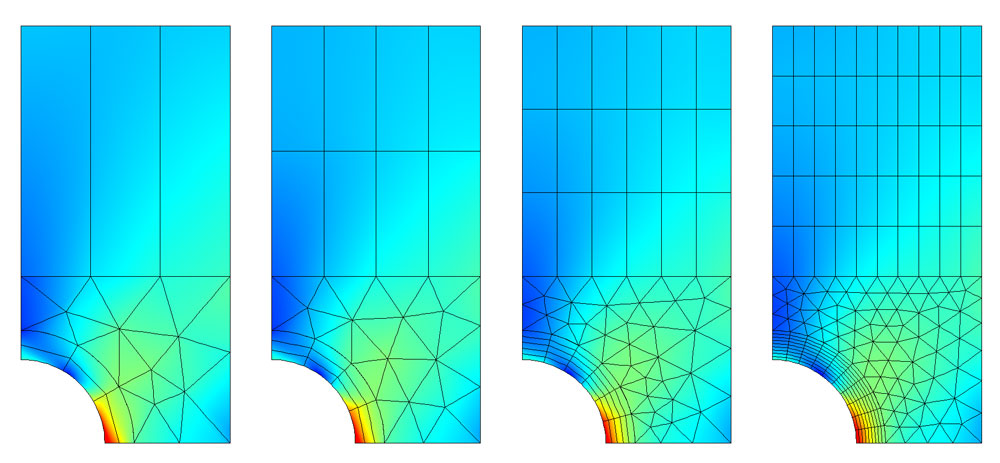
\includegraphics[width=0.68\textwidth]{Immagini/mesh-example.jpeg}
   \end{figure}}
\end{frame}

\begin{frame}{Elements}
   \begin{figure}[H]
    \centering
    \begin{tikzpicture}
        \scriptsize

        \node at (0,2) (A) {Discretization in different dimensions};
        \node at (-4,1.4) (B) {1D};
        \node at (0,1.4) (C) {2D};
        \node at (4,1.4) (D) {3D};

        \draw[->] (A) -- (C);
        \draw[->] (A) -- (-4,2) -- (B);
        \draw[->] (A) -- (4,2) -- (D);

        \node at (-4,0.7) (E) {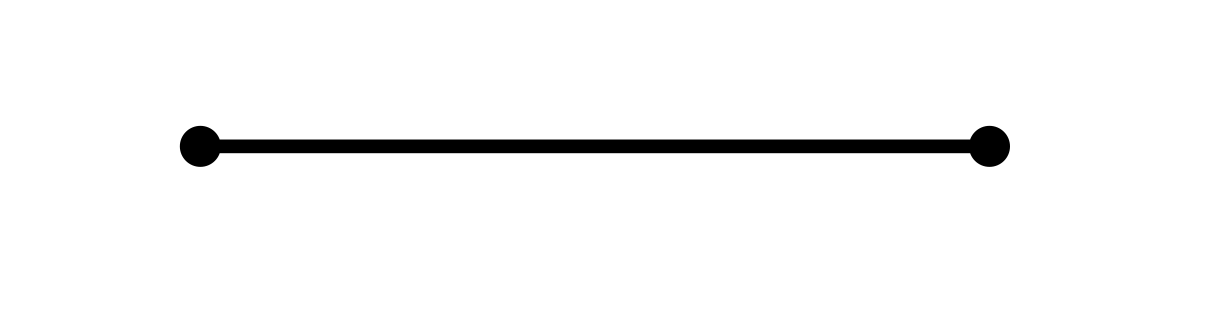
\includegraphics[width=0.218\textwidth]{Immagini/element-1D.png}};
        \node at (0,0.7) (F) {\includegraphics[width=0.2\textwidth]{Immagini/elements-2D.png}};
        \node at (4,0.68) (G) {\includegraphics[width=0.22\textwidth]{Immagini/elements-3D.png}};

        \visible<2->{\node at (-4,-1.8) (H) {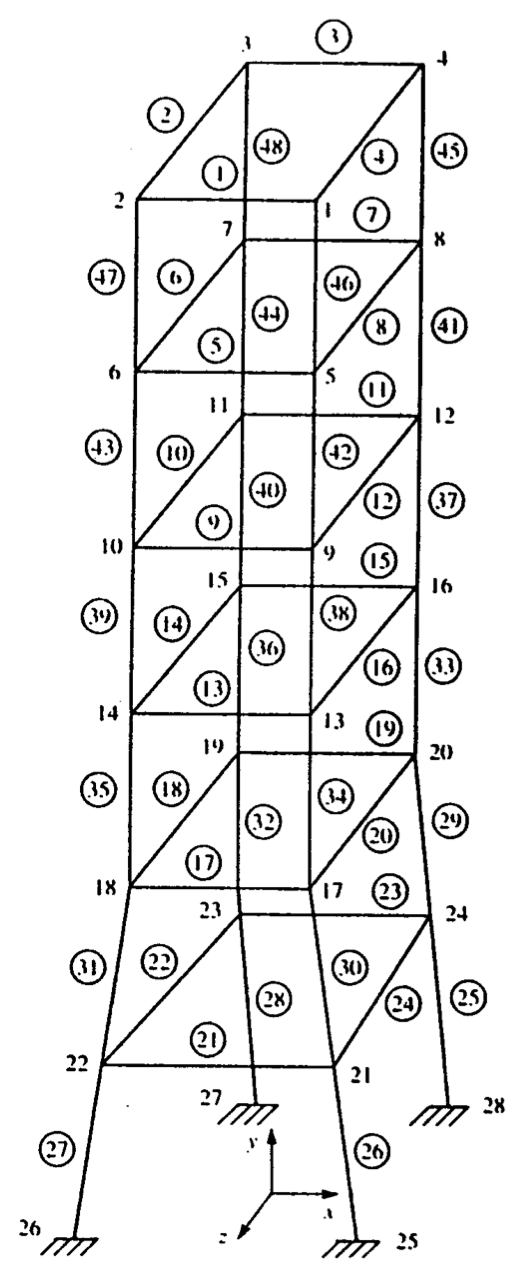
\includegraphics[width=0.14\textwidth]{Immagini/frame-elements.png}};
        \node at (-0.1,-1.9) (I) {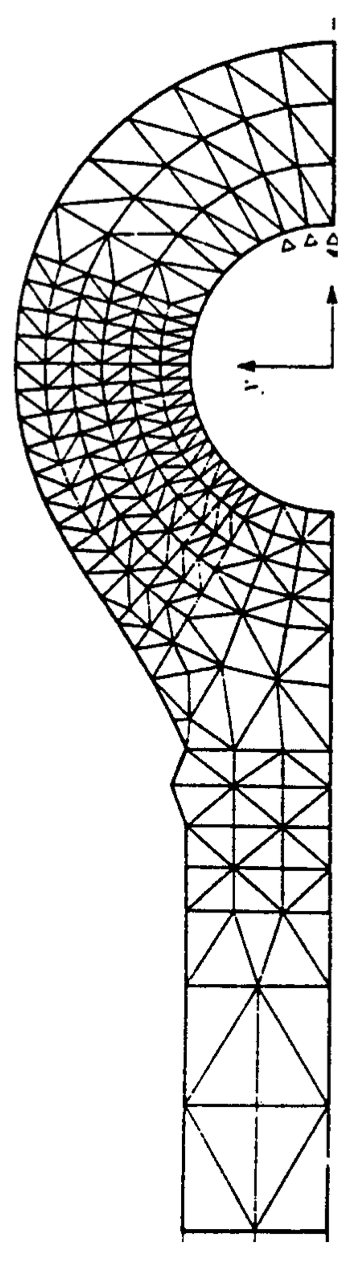
\includegraphics[width=0.1\textwidth]{Immagini/triangular elements.png}};
        \node at (3.78,-1.95) (J) {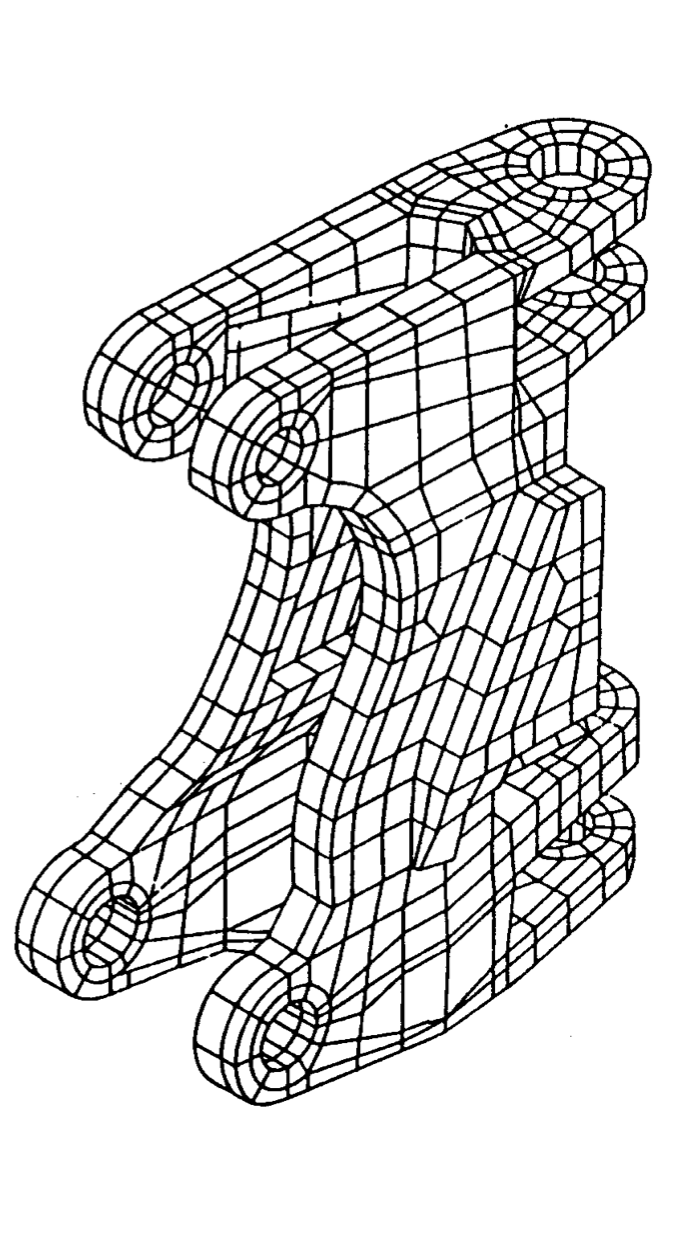
\includegraphics[width=0.21\textwidth]{Immagini/brick-elements.png}};

        \node at (-4,-4.1) (K) {\textbf{Frame \textcolor{BrickRed}{elements}}};
        \node at (0,-4.1) (L) {\textbf{Triangular \textcolor{BrickRed}{elements}}};
        \node at (4,-4.1) (M) {\textbf{Brick \textcolor{BrickRed}{elements}}};}

        \visible<3->{\draw[decorate, decoration={brace, amplitude=8pt, raise=2pt}] (5.25,-4.25) -- (-5.25,-4.25);

        \node at (0,-4.85) (N) {\textbf{Finite \textcolor{BrickRed}{Element} Method}};}

        \normalsize
    \end{tikzpicture}
\end{figure}
\end{frame}

\begin{frame}{Application examples}
   \begin{minipage}{0.5\textwidth}
      \begin{figure}[H]
         \raggedright
         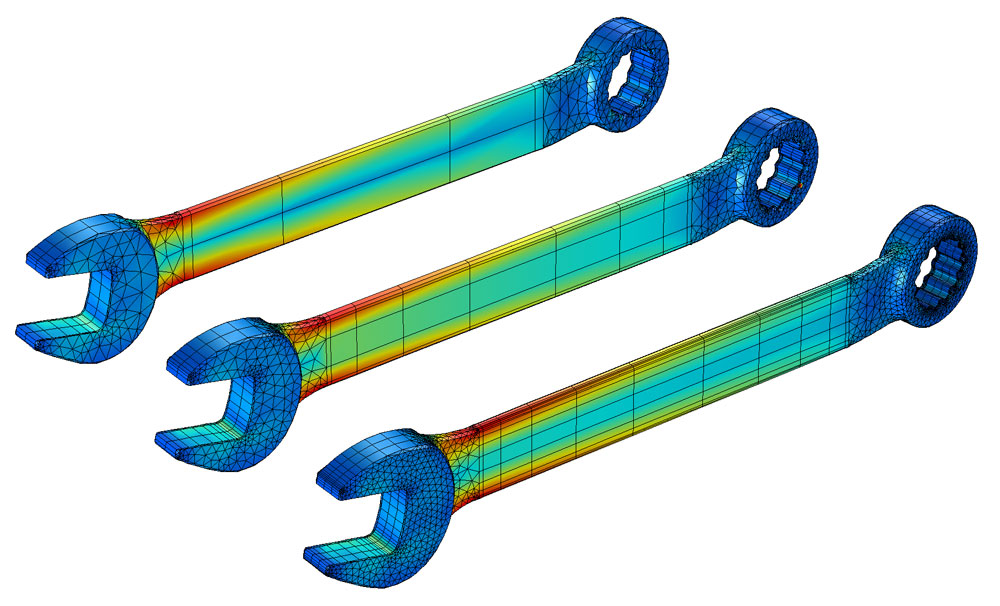
\includegraphics[width=\textwidth]{Immagini/mesh-application-1.jpeg}
      \end{figure}
   \end{minipage}
   \hfill
   \begin{minipage}{0.45\textwidth}
      \footnotesize{\textit{Manual mesh refinement of a wrench using different element types}}

      \textcolor{white}{some}

      \tiny{\texttt{Image from COMSOL Multiplysics Cyclopedia, ``Finite Element Mesh Refinement'', 21st of February 2017}}
   \end{minipage}

   \vfill

   \begin{minipage}{0.425\textwidth}
      \footnotesize{\textit{Mesh of a wheel rim composed of tetrahedrons in green, bricks in blue and prisms in pink}}

      \textcolor{white}{some}

      \tiny{\texttt{Image from COMSOL Multiplysics Blog, ``Meshing Your Geometry: When to Use the Various Element Types'', Walter Frei, 4th of November 2013}}
   \end{minipage}
   \hfill
   \begin{minipage}{0.5\textwidth}
      \begin{figure}[H]
         \raggedleft
         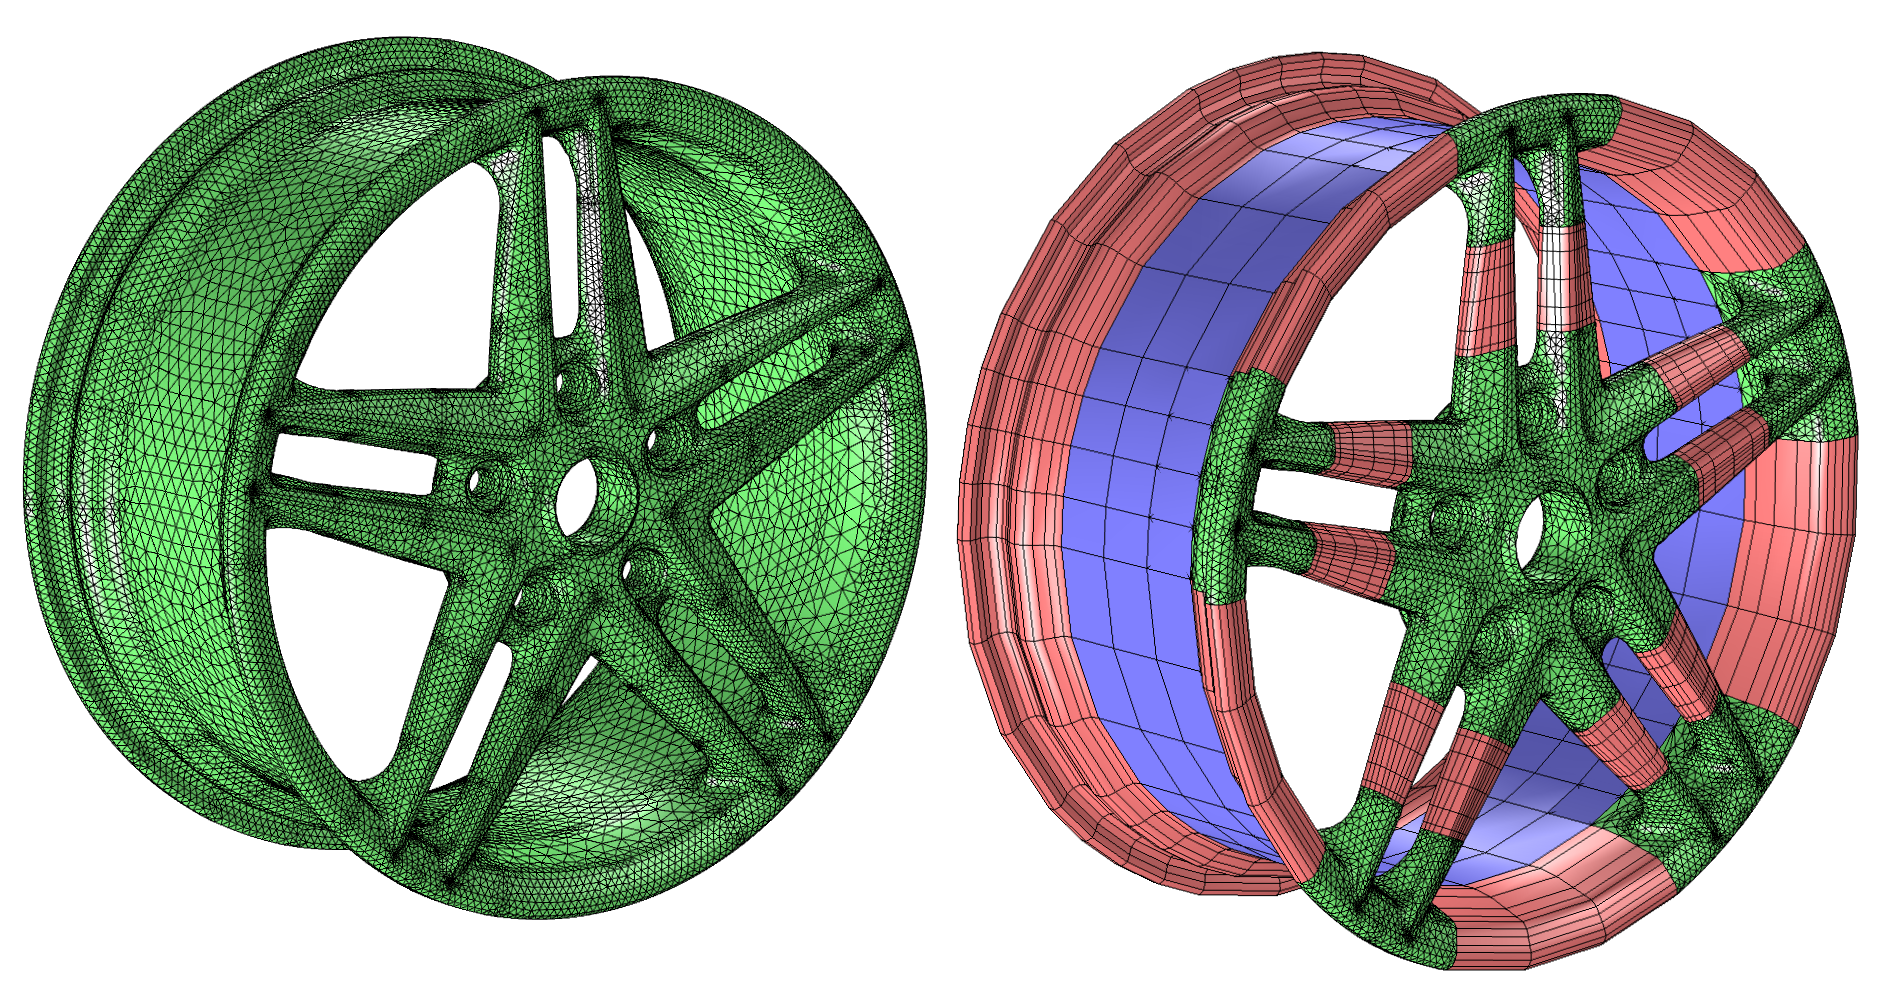
\includegraphics[width=\textwidth]{Immagini/mesh-application-2.png}
      \end{figure}
   \end{minipage}
\end{frame}

\begin{frame}{Choise of the base}
   \begin{figure}[H]
    \centering
    \begin{tikzpicture}
        \footnotesize

        \node at (0,2.4) (A) {Mesh division into sub-domains};

        \pause

        \draw[->] (0,2.05) -- (0,1.55);
        \node at (0,1.2) (B) {Choice of a \textbf{\textcolor{BrickRed}{local basis functions}}};

        \pause

        \draw[->] (0,0.85) -- (0,0.35);
        \node at (0,0) (C) {Exploitation of \underline{\textbf{compact support}}};

        \scriptsize

        \pause

        \node at (-3.458,-1.5) (D) {\textcolor{BrickRed}{$\bullet$} Leads to \textbf{sparse matrices}};
        \node at (-3.376,-2.25) (E) {\textcolor{BrickRed}{$\bullet$} Allows \textbf{local interpolation}};
        \node at (-3.174,-3) (F) {\textcolor{BrickRed}{$\bullet$} Enhances \textbf{numerical stability}};
        \node at (-3,-3.75) (G) {\textcolor{BrickRed}{$\bullet$} Enables \textbf{efficient parallelization}};

        \draw[->] (C) -- (-3.458,0) -- (D);

        \visible<4->{\node at (2.795,-2.58) (H) {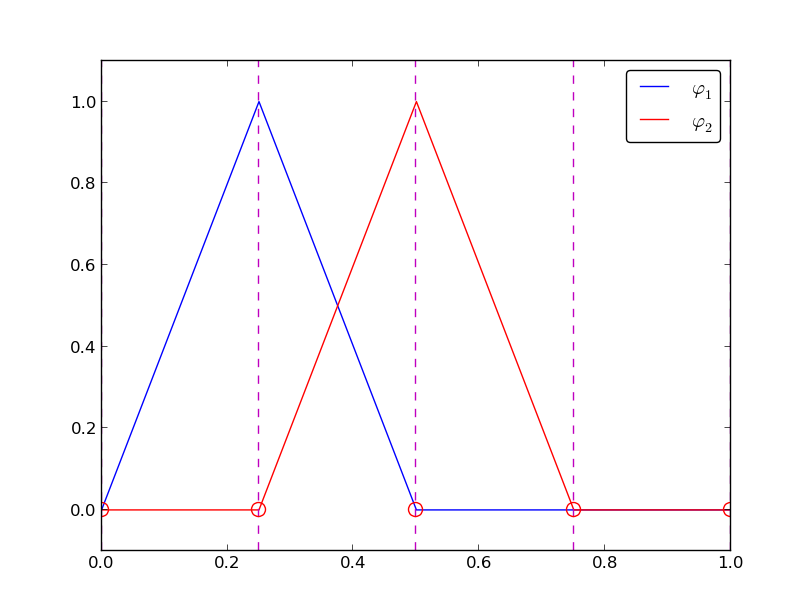
\includegraphics[width=0.45\textwidth]{Immagini/local-basis-functions.png}};}

        \normalsize
    \end{tikzpicture}
\end{figure}
\end{frame}

\subsection{Introduction to FEniCS}

\begin{frame}{FEniCS library}
   \small{A leading software platform for finite element computations is \textbf{\textcolor{BrickRed}{FEniCS}}.}

   \vfill

   \pause

   \scriptsize

   \begin{minipage}{0.38\textwidth}
      \begin{itemize}
         \item \textbf{Open-source} and freely available
         \item \textbf{Multi-language support} (\texttt{C++} and \texttt{Python} APIs)
         \item \textbf{Parallel computing} with MPI support
      \end{itemize}
   \end{minipage}
   \hfill
   \visible<2->{\begin{minipage}{0.57\textwidth}
      \begin{figure}[H]
         \centering
         
\includegraphics[width=\textwidth]{Immagini/fenics-logo.png}
      \end{figure}
   \end{minipage}}

   \vfill

   \pause

   \small

   \begin{equation*}
      \text{\texttt{FEniCS} package:}
      \begin{cases}
         \text{\texttt{DOLFIN}} \ &\text{(backend core engine and \texttt{PETSc} interface)}\\
         \text{\texttt{UFL}} \ &\text{(symbolic language)}\\
         \text{\texttt{FIAT}} \ &\text{(shape functions tabulator)}\\
         \text{\texttt{FFC}} \ &\text{(\texttt{C++} compiler for efficient local assembly)}\\
         \text{\texttt{MSHR}} \ &\text{(mesh generator)}
      \end{cases}
   \end{equation*}

   \normalsize
\end{frame}

\begin{frame}{A minimal FEniCS example: setup}
   \small{Setup of a \underline{Poisson equation} with Neumann boundary conditions in \texttt{FEniCS}:}

   \vspace{0.2cm}

   \begin{itemize}
      \item \small{Generation of the mesh}
      
      \begin{tcolorbox}[pythoncode]
         \footnotesize{\texttt{\textcolor{cyan!60!black}{domain} = \textcolor{violet!80!black}{mesh}.\textcolor{green!40!black}{create\_interval}(\textcolor{violet!80!black}{MPI}.\textcolor{green!40!black}{COMM\_WORLD}, \textcolor{cyan!60!black}{nx}, [\textcolor{brown!70!black}{0.0}, \textcolor{cyan!60!black}{L}])}}
      \end{tcolorbox}

      \item \small{Definition of the finite element function space}
      
      \begin{tcolorbox}[pythoncode]
         \footnotesize{\texttt{\textcolor{cyan!60!black}{V} = \textcolor{green!40!black}{functionspace}(\textcolor{cyan!60!black}{domain}, (\textcolor{red!80!black}{"Lagrange"}, \textcolor{brown!70!black}{1}))}}
      \end{tcolorbox}

      \item \small{Definition of trial function and test function}
      
      \begin{tcolorbox}[pythoncode]
         \footnotesize{\texttt{\textcolor{cyan!60!black}{u} = \textcolor{violet!80!black}{ufl}.\textcolor{green!40!black}{TrialFunction}(\textcolor{cyan!60!black}{V})}}

         \footnotesize{\texttt{\textcolor{cyan!60!black}{v} = \textcolor{violet!80!black}{ufl}.\textcolor{green!40!black}{TestFunction}(\textcolor{cyan!60!black}{V})}}
      \end{tcolorbox}

      \item \small{Definition of the source term}
      
      \begin{tcolorbox}[pythoncode]
         \footnotesize{\texttt{\textcolor{cyan!60!black}{f} = \textcolor{violet!80!black}{fem}.\textcolor{green!40!black}{Constant}(\textcolor{cyan!60!black}{domain}, \textcolor{green!40!black}{default\_scalar\_type}(\textcolor{brown!70!black}{-6}))}}
      \end{tcolorbox}
   \end{itemize}
\end{frame}

\begin{frame}{A minimal FEniCS example: solution}
   \small{Solving \underline{Poisson equation} with Neumann boundary conditions in \texttt{FEniCS}:}

   \vspace{0.2cm}

   \begin{itemize}
      \item \small{Weak formulation}
      
      \begin{tcolorbox}[pythoncode]
         \footnotesize{\texttt{\textcolor{cyan!60!black}{a} = \textcolor{violet!80!black}{ufl}.\textcolor{green!40!black}{dot}(\textcolor{violet!80!black}{ufl}.\textcolor{green!40!black}{grad}(\textcolor{cyan!60!black}{u}), \textcolor{violet!80!black}{ufl}.\textcolor{green!40!black}{grad}(\textcolor{cyan!60!black}{v})) * \textcolor{violet!80!black}{ufl}.\textcolor{green!40!black}{dx}}}

         \footnotesize{\texttt{\textcolor{cyan!60!black}{F} = \textcolor{cyan!60!black}{f} * \textcolor{cyan!60!black}{v} * \textcolor{violet!80!black}{ufl}.\textcolor{green!40!black}{dx}}}
      \end{tcolorbox}

      \item \small{Solution of the linear system}
      
      \begin{tcolorbox}[pythoncode]
         \footnotesize{\texttt{\textcolor{cyan!60!black}{problem} = \textcolor{green!40!black}{LinearProblem}(\textcolor{cyan!60!black}{a}, \textcolor{cyan!60!black}{F},}}
         
         \footnotesize{\texttt{\textcolor{gray!10}{aaaaaaaaaaaaaaaaaaaaaaaa}\textcolor{cyan!60!black}{petsc\_option} = \{\textcolor{red!80!black}{"ksp\_type"}: \textcolor{red!80!black}{"preonly"},}}
         
         \footnotesize{\texttt{\textcolor{gray!10}{aaaaaaaaaaaaaaaaaaaaaaaaaaaaaaaaaaaaaaaa}\textcolor{red!80!black}{"pc\_type"} : \textcolor{red!80!black}{"lu"}}}
         
         \footnotesize{\texttt{\textcolor{gray!10}{aaaaaaaaaaaaaaaaaaaaaaaaaaaaaaaaaaaaaa} \}}}
         
         \footnotesize{\texttt{\textcolor{gray!10}{aaaaaaaaaaaaaaaaaaaaaaa})}}

         \footnotesize{\texttt{\textcolor{cyan!60!black}{u\_h} = \textcolor{cyan!60!black}{problem}.\textcolor{green!40!black}{solve}()}}
      \end{tcolorbox}
   \end{itemize}

   \vfill
\end{frame}

\section{Classical Wave Equation}

\begin{frame}{Approach to the classical wave equation}
    Our first goal is to approximate the solution of

    \begin{equation*}
        \fcolorbox{BrickRed}{white}{$\displaystyle\frac{\partial^2u}{\partial t^2}-c^2\frac{\partial^2u}{\partial x^2}=0$} \ \longleftarrow \ \text{\textbf{\textcolor{BrickRed}{d'Alembert equation}}}
    \end{equation*}

    \vfill

    \pause

    \begin{figure}[H]
    \centering
    \begin{tikzpicture}
        \node at (0,3) (A) {\underline{Separate} discretization};
        \node at (-3.15,1.8) (B) {Spatial part};
        \node at (3.15,1.8) (C) {Temporal part};
        \node at (-3.15,0.6) (D) {\small{\textbf{Finite Element Method}}};
        \node at (3.15,0.6) (E) {\small{\textbf{Finite Difference Method}}};
        \node at (-3.15,-0.3) (F) {\tiny{$\displaystyle\int_0^L\frac{\partial^2u}{\partial x^2}vdx=\frac{\partial u}{\partial x}v\bigg|_0^L-\int_0^L\frac{\partial u}{\partial x}\frac{\partial v}{\partial x}dx$}};
        \node at (3.15,-0.3) (G) {\tiny{$\displaystyle\frac{\partial^2u}{\partial t^2}\simeq\frac{u^{(n+1)}-2u^{(n)}+u^{(n-1)}}{\Delta t^2}$}};

        \draw[->] (A) -- (-3.15,3) -- (B);
        \draw[->] (A) -- (3.15,3) -- (C);
        \draw[->] (B) -- (D);
        \draw[->] (C) -- (E);

        \draw[white] (3.2,-1) -- (3.2,0);
    \end{tikzpicture}
\end{figure}
\end{frame}

\begin{frame}{From PDE to ODEs}
    To do so, a \textbf{separable base} must be chosen:

    \begin{equation*}
        u_h(x,t)=\sum_{j=1}^Nu_j(t)\phi_j(x)
    \end{equation*}

    \vfill

    \pause

    Managing the boundary term separately, the weak formulation goes as

    \small

    \begin{equation*}
        \int_0^L\frac{\partial^2\textcolor{RoyalBlue}{u}}{\partial t^2}\textcolor{ForestGreen}{v}dx+c^2\int_0^L\frac{\partial\textcolor{RoyalBlue}{u}}{\partial x}\frac{\partial\textcolor{ForestGreen}{v}}{\partial x}dx=0 \qquad \forall v\in H^1([0,L])
    \end{equation*}

    \pause

    \begin{equation*}
        \Big\Downarrow
    \end{equation*}

    \vspace{-0.35cm}

    \begin{equation*}
        \textcolor{RoyalBlue}{\sum_{j=1}^N}\frac{d^2\textcolor{RoyalBlue}{u_j}}{dt^2}\int_0^L\textcolor{RoyalBlue}{\phi_j}\textcolor{ForestGreen}{\phi_i}dx+c^2\textcolor{RoyalBlue}{\sum_{j=1}^Nu_j}\int_0^L\frac{\partial\textcolor{RoyalBlue}{\phi_j}}{\partial x}\frac{\partial\textcolor{ForestGreen}{\phi_i}}{\partial x}dx=0 \qquad \forall i=1,\dots,N
    \end{equation*}

    \normalsize
\end{frame}

\begin{frame}{Matrix formulation}
    Let's define

    \begin{alignat*}{3}
        M&:M_{i,j}&&=\int_0^L\phi_j\phi_idx \ &&\longleftarrow \ \text{\textbf{\textcolor{BrickRed}{Mass matrix}}}\\
        A&:A_{i,j}&&=\int_0^L\frac{\partial\phi_j}{\partial x}\frac{\partial\phi_i}{\partial x}dx \ &&\longleftarrow \ \text{\textbf{\textcolor{BrickRed}{Stiffness matrix}}}
    \end{alignat*}

    \pause

    \begin{equation*}
        \Big\Downarrow
    \end{equation*}

    \begin{equation*}
        \fcolorbox{BrickRed}{white}{\text{$\displaystyle M\frac{d^2\boldsymbol{u}}{dt^2}+c^2A\boldsymbol{u}=0$}}
    \end{equation*}
\end{frame}

\begin{frame}{Time discretization}
    Let's apply \textbf{\textcolor{BrickRed}{implicit} central difference scheme}:

    \begin{equation*}
        M\frac{\boldsymbol{u}^{(n+1)}-2\boldsymbol{u}^{(n)}+\boldsymbol{u}^{(n-1)}}{\Delta t^2}+c^2A\boldsymbol{u}^{\textcolor{BrickRed}{(n+1)}}=0
    \end{equation*}

    \pause

    \begin{equation*}
        \Big\Downarrow
    \end{equation*}

    \begin{equation*}
        \fcolorbox{BrickRed}{white}{\text{$\displaystyle\left(\frac{1}{\Delta t^2}M+c^2A\right)\boldsymbol{u}^{(n+1)}=\frac{2}{\Delta t^2}M\boldsymbol{u}^{(n)}-\frac{1}{\Delta t^2}M\boldsymbol{u}^{(n-1)}$}}
    \end{equation*}
\end{frame}

\begin{frame}{Analytical solutions}
    Solutions are known since 1747 due to d'Alembert himself.

    \vfill

    \alt<1>{\begin{itemize}
        \item \textbf{Dirichlet} boundary conditions: $\displaystyle u(0,t)=u(L,t)=0$
        
        \vspace{0.1cm}
        
        \begin{equation*}
            \fcolorbox{BrickRed}{white}{\text{$\displaystyle u(x,t)=\sum_{n=1}^\infty A_n\cos\left(\frac{n\pi}{L}ct\right)\sin\left(\frac{n\pi}{L}x\right)$}}
        \end{equation*}

        with $A_n=\frac{2}{L}\int_0^Lf(x)\sin\left(\frac{n\pi}{L}x\right)dx$.

        \vfill

        \begin{figure}[H]
            \centering
            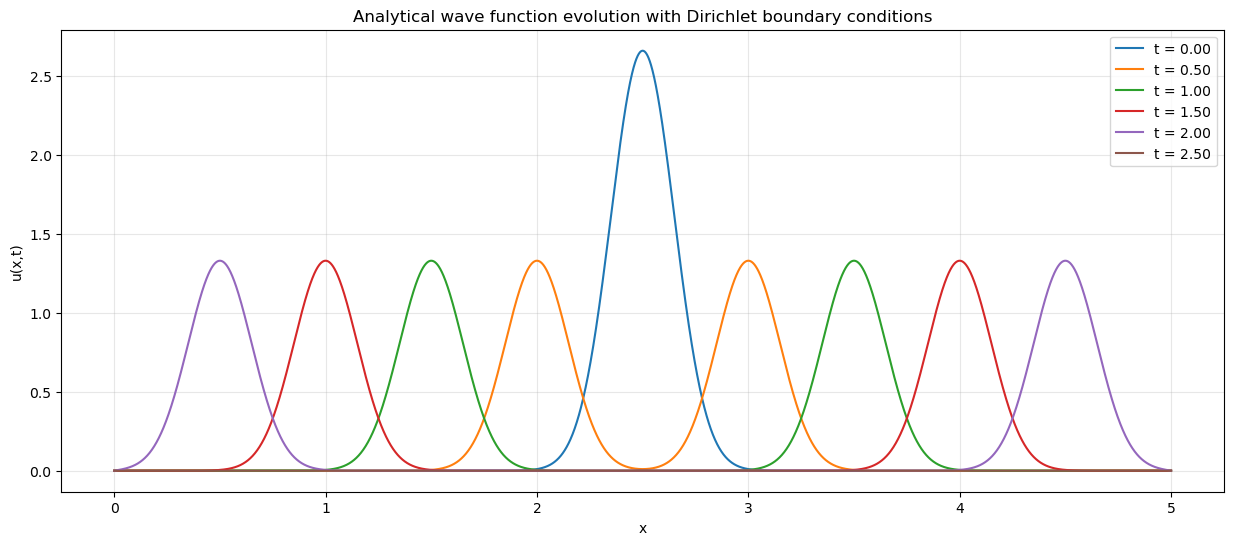
\includegraphics[width=0.8\textwidth]{Immagini/plot-dirichlet-analytical.png}
        \end{figure}
    \end{itemize}}{}

    \alt<2>{\begin{itemize}
        \item \textbf{Neumann} boundary conditions: \small{$\displaystyle\frac{\partial u}{\partial x}\bigg|_{x=0}=\frac{\partial u}{\partial x}\bigg|_{x=L}=0$}
        
        \vspace{0.1cm}

        \normalsize
        
        \begin{equation*}
            \fcolorbox{BrickRed}{white}{\text{$\displaystyle u(x,t)=A_0+\sum_{n=1}^\infty A_n\cos\left(\frac{n\pi}{L}ct\right)\cos\left(\frac{n\pi}{L}x\right)$}}
        \end{equation*}

        with $A_0=\frac{1}{L}\int_0^Lf(x)dx$, $A_n=\frac{2}{L}\int_0^Lf(x)\cos\left(\frac{n\pi}{L}x\right)dx$.

        \vfill

        \begin{figure}[H]
            \centering
            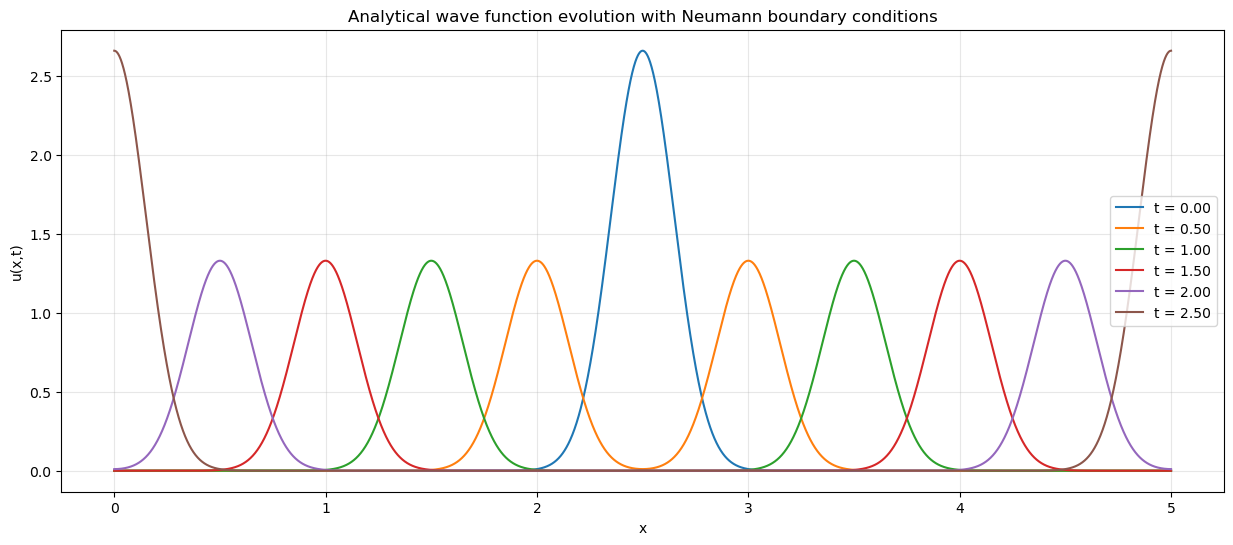
\includegraphics[width=0.8\textwidth]{Immagini/plot-neumann-analytical.png}
        \end{figure}
    \end{itemize}}{}
\end{frame}

\begin{frame}{Approximate solutions}
    \small

    The selection of discretization steps should\normalsize{$^{\boldsymbol{\textcolor{BrickRed}{\ast}}}$} \small{take into account}

    \begin{equation*}
        \text{\textbf{\textcolor{BrickRed}{CFL} stability condition}}: \ \frac{c\Delta t}{\Delta x}\lesssim1
    \end{equation*}

    \small

    \uncover<2>{\begin{center}
        Choosing \underline{first-order Lagrange polynomials} as $\left\{\phi_i\right\}$:
    \end{center}}

    \vfill

    \normalsize

    \visible<2>{\begin{minipage}{0.49\textwidth}
        \begin{center}
            \small{\textbf{Dirichlet}}
        \end{center}

        \vspace{-0.2cm}

        \begin{figure}[H]
            \centering
            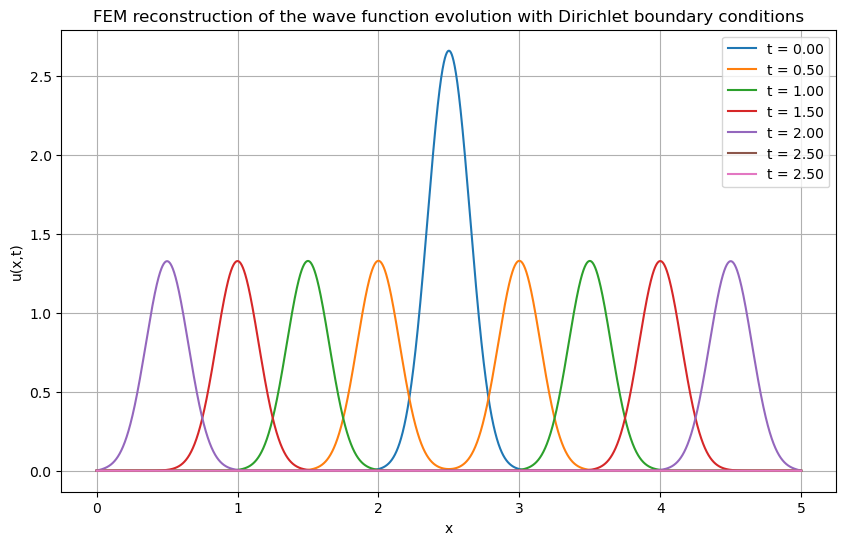
\includegraphics[width=\textwidth]{Immagini/plot-dirichlet-approximated.png}
        \end{figure}
    \end{minipage}
    \hfill
    \begin{minipage}{0.49\textwidth}
        \begin{center}
            \small{\textbf{Neumann}}
        \end{center}

        \vspace{-0.2cm}

        \begin{figure}[H]
            \centering
            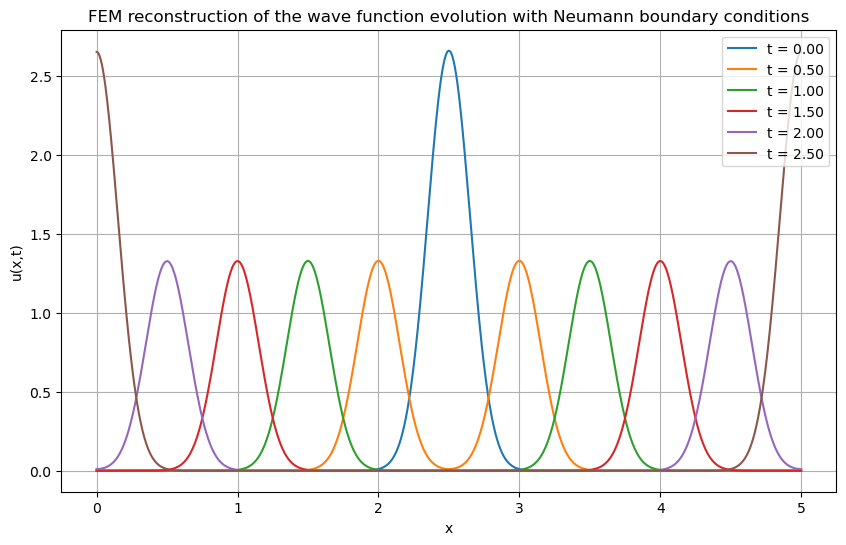
\includegraphics[width=\textwidth]{Immagini/plot-neumann-approximated.png}
        \end{figure}
    \end{minipage}}

    \vfill

    $^{\boldsymbol{\textcolor{BrickRed}{\ast}}}$\scriptsize{While for implicit schemes it is only a recommendation, for explicit ones it is \underline{mandatory}.}

    \normalsize
\end{frame}

\begin{frame}{Energy loss}
    \small

    A strong indicator of numerical correctness is \textbf{\underline{energy conservation}}.

    \pause

    \begin{equation*}
        \text{\textbf{\textcolor{BrickRed}{Energy}}:} \ E=\underbrace{\frac{T}{2c^2}\int_0^L\left(\frac{\partial u}{\partial t}\right)^2dx}_{\text{Kinetic}}+\underbrace{\frac{T}{2}\int_0^L\left(\frac{\partial u}{\partial x}\right)^2dx}_{\text{Potential}}
    \end{equation*}

    $T$ is the \textit{tension}, which can be arbitrarily set to $1$.

    \vfill

    \scriptsize

    \visible<3>{\begin{minipage}{0.32\textwidth}
        \begin{equation*}
            \text{CFL}=0.05
        \end{equation*}

        \vspace{-0.2cm}

        \begin{figure}[H]
            \centering
            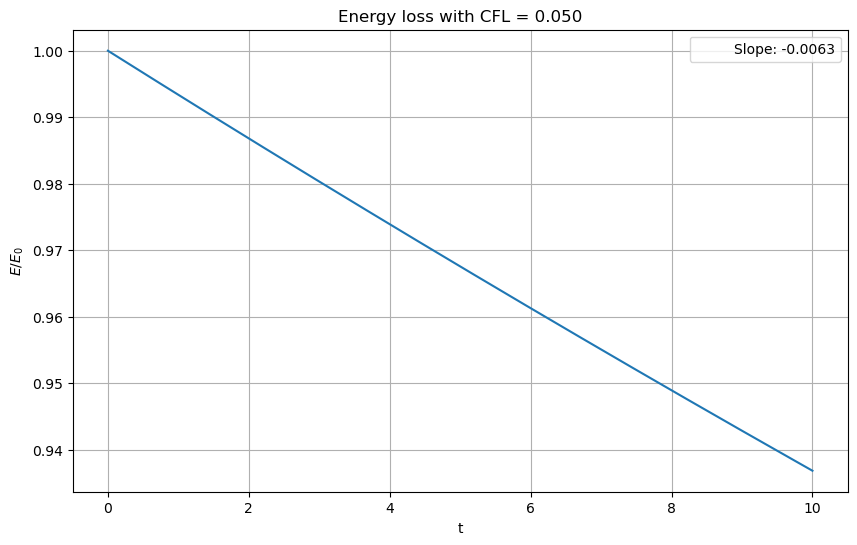
\includegraphics[width=\textwidth]{Immagini/plot-energy-decay-cfl-0.05.png}
        \end{figure}
    \end{minipage}
    \hfill
    \begin{minipage}{0.32\textwidth}
        \begin{equation*}
            \text{CFL}=0.25
        \end{equation*}

        \vspace{-0.2cm}

        \begin{figure}[H]
            \centering
            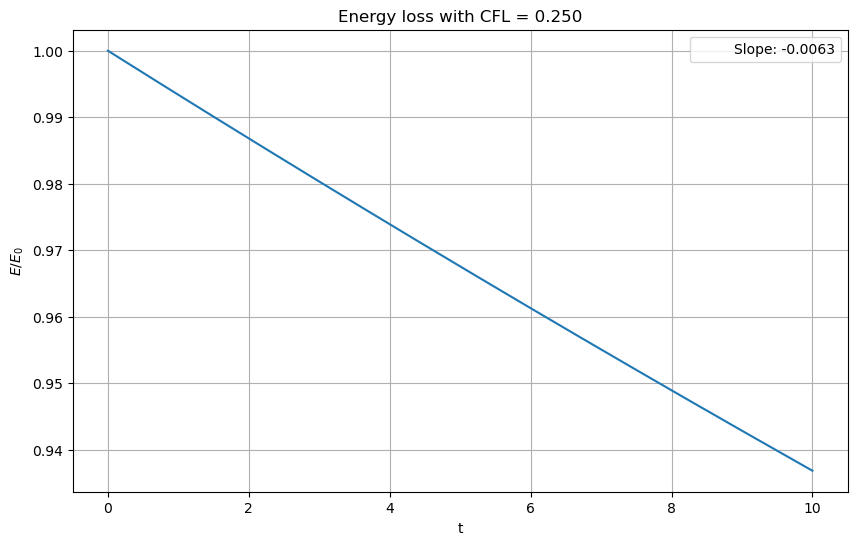
\includegraphics[width=\textwidth]{Immagini/plot-energy-decay-cfl-0.25.png}
        \end{figure}
    \end{minipage}
    \hfill
    \begin{minipage}{0.32\textwidth}
        \begin{equation*}
            \text{CFL}=0.50
        \end{equation*}

        \vspace{-0.2cm}

        \begin{figure}[H]
            \centering
            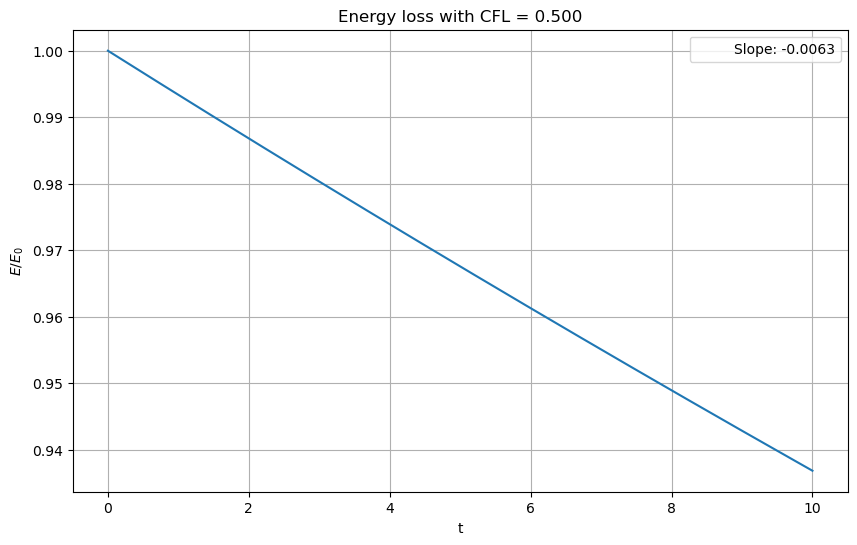
\includegraphics[width=\textwidth]{Immagini/plot-energy-decay-cfl-0.50.png}
        \end{figure}
    \end{minipage}}

    \vfill

    \footnotesize

    \pause

    Numerical energy decay is \textit{independent} of the CFL number, being entirely caused by the \textbf{implicit scheme} itself.

    \normalsize
\end{frame}

\begin{frame}{What if $c=c(x)$?}
    If $c$ is not constant, its square must be interpolated as the wave function:

    \begin{equation*}
        c(^2x) \ \longrightarrow \ c_h^2(x)=\sum_{k=1}^Nc_k^{(2)}\psi_k(x)
    \end{equation*}

    \pause

    Velocity must be included in the stiffness matrix $A$:

    \begin{equation*}
        A_{i,j}=\int_0^L\left(\sum_{k=1}^Nc_k^{(2)}\psi_k(x)\right)\frac{\partial\phi_j}{\partial x}\frac{\partial\phi_i}{\partial x}dx
    \end{equation*}

    \pause

    \begin{equation*}
        \Big\Downarrow
    \end{equation*}

    \begin{equation*}
        \fcolorbox{BrickRed}{white}{\text{$\displaystyle M\frac{d^2\boldsymbol{u}}{dt^2}+A\boldsymbol{u}=0$}}
    \end{equation*}
\end{frame}

\begin{frame}{Piecewise constant velocity}
    \small

    One simple example is the \textbf{piacewise constant function}:

    \begin{equation*}
        c(x)=
        \begin{cases}
            c_1 \ \ \  &x\leqslant x_0\\
            c_2 \ \ \  &x>x_0
        \end{cases}
    \end{equation*}

    \vfill

    \alt<1>{\begin{center}
        Placing initial pulse \underline{on the left} with \textcolor{RoyalBlue}{$\boldsymbol{c_1=1}$}, \textcolor{RoyalBlue}{$\boldsymbol{c_2=3}$}:
    \end{center}

    \vspace{0.2cm}

    \begin{minipage}{0.49\textwidth}
        \begin{center}
            \textcolor{RoyalBlue}{\textbf{Dirichlet}}
        \end{center}

        \vspace{-0.3cm}

        \begin{figure}[H]
            \centering
            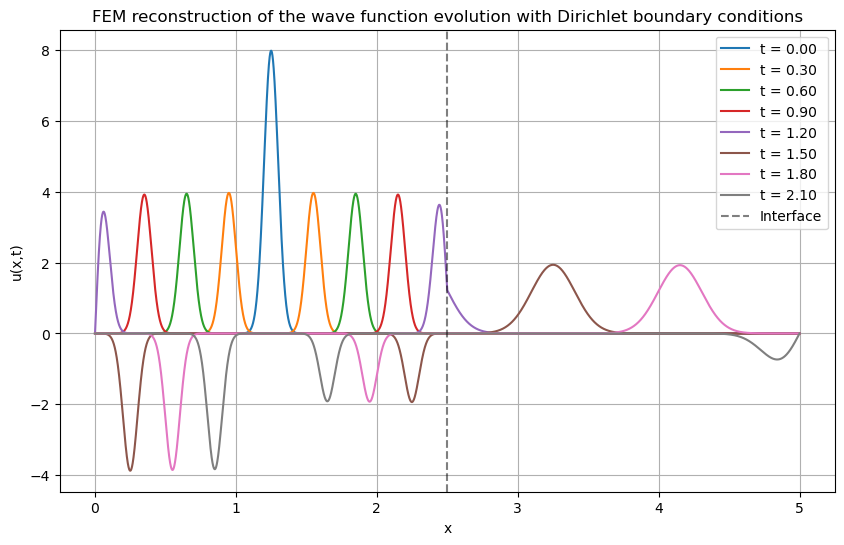
\includegraphics[width=\textwidth]{Immagini/plot-dirichlet-piecewise-c1<c2.png}
        \end{figure}
    \end{minipage}
    \hfill
    \begin{minipage}{0.49\textwidth}
        \begin{center}
            \textcolor{RoyalBlue}{\textbf{Neumann}}
        \end{center}

        \vspace{-0.3cm}

        \begin{figure}[H]
            \centering
            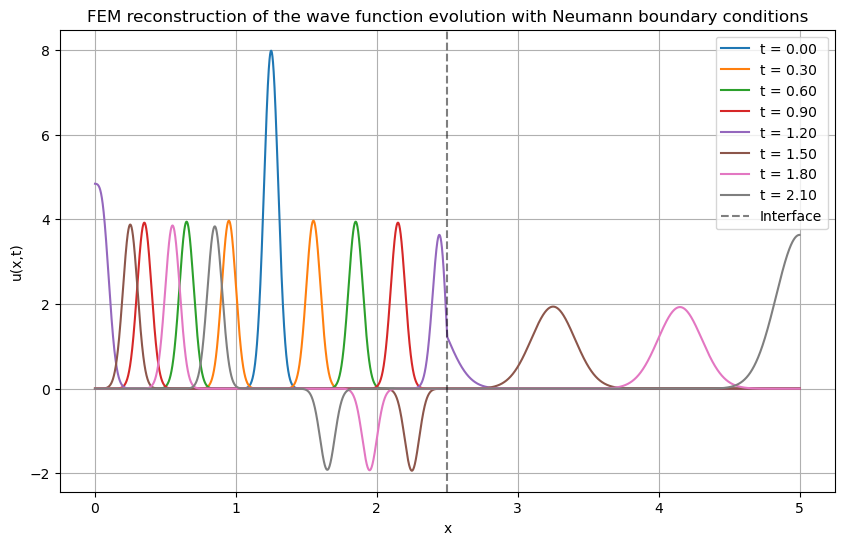
\includegraphics[width=\textwidth]{Immagini/plot-neumann-piecewise-c1<c2.png}
        \end{figure}
    \end{minipage}}{}

    \alt<2>{\begin{center}
        Placing initial pulse \underline{on the left} with \textcolor{ForestGreen}{$\boldsymbol{c_1=3}$}, \textcolor{ForestGreen}{$\boldsymbol{c_2=1}$}:
    \end{center}

    \vspace{0.2cm}

    \begin{minipage}{0.49\textwidth}
        \begin{center}
            \textcolor{ForestGreen}{\textbf{Dirichlet}}
        \end{center}

        \vspace{-0.3cm}

        \begin{figure}[H]
            \centering
            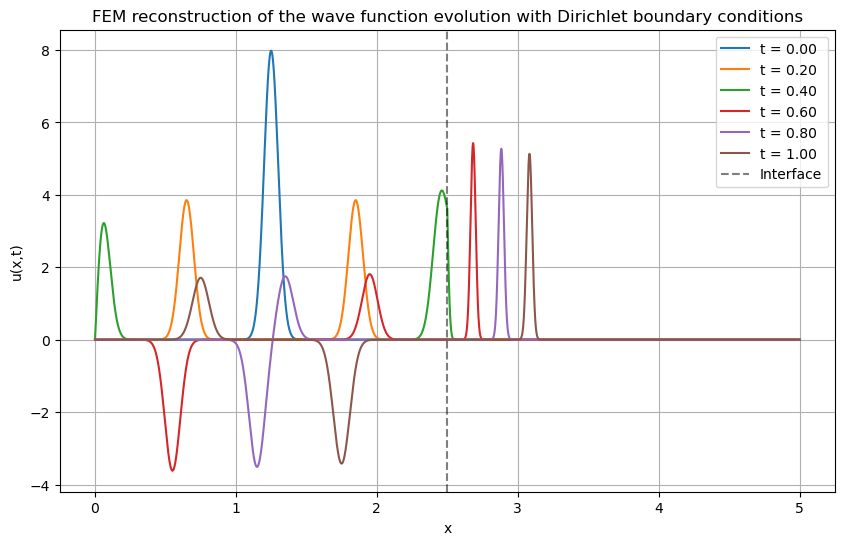
\includegraphics[width=\textwidth]{Immagini/plot-dirichlet-piecewise-c1>c2.png}
        \end{figure}
    \end{minipage}
    \hfill
    \begin{minipage}{0.49\textwidth}
        \begin{center}
            \textcolor{ForestGreen}{\textbf{Neumann}}
        \end{center}

        \vspace{-0.3cm}

        \begin{figure}[H]
            \centering
            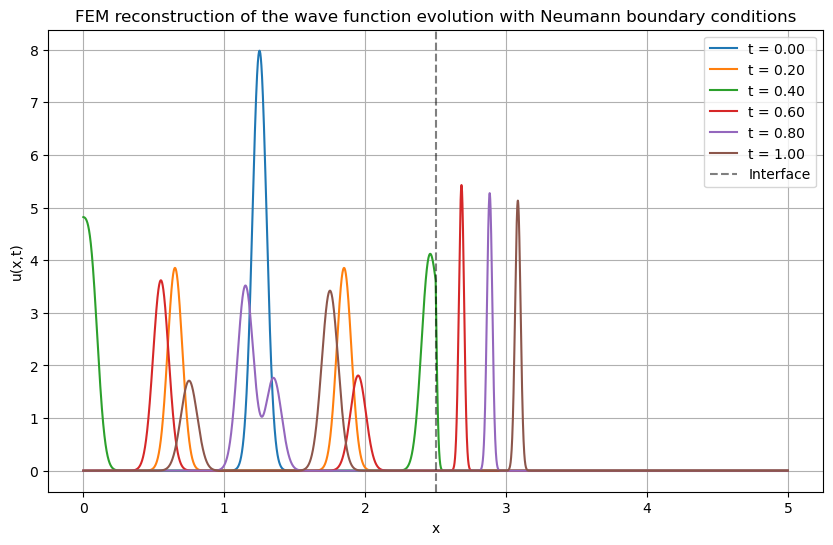
\includegraphics[width=\textwidth]{Immagini/plot-neumann-piecewise-c1>c2.png}
        \end{figure}
    \end{minipage}}{}

    \normalsize
\end{frame}

\begin{frame}{Fresnel coefficients}
    \small

    In this case, the analytical reference values are the \textcolor{BrickRed}{\textbf{Fresnel coefficients}}.

    \normalsize

    \begin{equation*}
        T=\frac{2c_1}{c_1+c_2} \hspace{1cm} R=\frac{c_1-c_2}{c_1+c_2}
    \end{equation*}
\end{frame}

\begin{frame}{Approach to the Schrödinger equation}
    Moving in the quantum realm, 
\end{frame}

\section{Time-Dependent Schrödinger Equation}

\begin{frame}{Approach to the Schrödinger equation}
    Moving in the quantum realm, our next goal is to approximate the solution of a \textbf{1D time-dependent \textcolor{BrickRed}{Schrödinger equation}}:

    \begin{equation*}
        \fcolorbox{BrickRed}{white}{\text{$\displaystyle i\hbar\frac{\partial\psi}{\partial t}=-\frac{\hbar^2}{2m}\frac{\partial^2\psi}{\partial x^2}+V(x)\psi(x,t)$}}
    \end{equation*}

    \pause

    \begin{equation*}
        \Big\Downarrow
    \end{equation*}

    \small

    \begin{equation*}
        \underbrace{i\hbar\sum_{j=1}^N\frac{d\psi_j}{dt}\int_{-L}^L\phi_j\phi_idx}_{i\hbar M\frac{d\boldsymbol{\psi}}{dt}}=\underbrace{\frac{\hbar^2}{2m}\sum_{j=1}^N\psi_j\int_{-L}^L\frac{\partial\phi_j}{\partial x}\frac{\partial\phi_i}{\partial x}dx}_{\frac{\hbar^2}{2m}A\boldsymbol{\psi}}+\sum_{j=1}^N\psi_j\int_{-L}^LV\phi_j\phi_idx
    \end{equation*}

    \normalsize
\end{frame}

\begin{frame}{Potential matrix}
    In the equation it appears a \underline{linear term}.

    \pause
    
    We must then introduce a new matrix, that can be called \textcolor{BrickRed}{\textbf{potential matrix}}, which is nothing different than a \textbf{weighted mass matrix}:

    \begin{equation*}
        V:V_{i,j}=\int_\Omega V(x)\phi_j(x)\phi_i(x)dx
    \end{equation*}

    \pause

    \begin{equation*}
        \Big\Downarrow
    \end{equation*}

    \begin{equation*}
        i\hbar M\frac{d\boldsymbol{\psi}}{dt}=\frac{\hbar^2}{2m}A\boldsymbol{\psi}+V\boldsymbol{\psi}
    \end{equation*}

    \pause

    \begin{equation*}
        \Big\Downarrow
    \end{equation*}

    \begin{equation*}
        \fcolorbox{BrickRed}{white}{\text{$\displaystyle M\frac{d\boldsymbol{\psi}}{dt}=-\frac{i}{\hbar}\left(\frac{\hbar^2}{2m}A+V\right)\boldsymbol{\psi}$}}
    \end{equation*}
\end{frame}

\begin{frame}{Application of the Cranck-Nicholson method}
    In this case, the PDE is of \underline{first order} in time.

    \pause

    The most suitable method to use is the \textcolor{BrickRed}{\textbf{Crank-Nicholson}} scheme:

    \begin{equation*}
        M\frac{\boldsymbol{\psi}^{(n+1)}-\boldsymbol{\psi}^{(n)}}{\Delta t}=-\frac{i}{2\hbar}\left(\frac{\hbar^2}{2m}A+V\right)\boldsymbol{\psi}^{(n+1)}-\frac{i}{2\hbar}\left(\frac{\hbar^2}{2m}A+V\right)\boldsymbol{\psi}^{(n)}
    \end{equation*}

    \pause

    \begin{equation*}
        \Big\Downarrow
    \end{equation*}

    \begin{equation*}
        \fcolorbox{BrickRed}{white}{\text{$\displaystyle\left[M+\frac{i\Delta t}{2\hbar}\left(\frac{\hbar^2}{2m}A+V\right)\right]\boldsymbol{\psi}^{(n+1)}=\left[M-\frac{i\Delta t}{2\hbar}\left(\frac{\hbar^2}{2m}A+V\right)\right]\boldsymbol{\psi}^{(n)}$}}
    \end{equation*}
\end{frame}

\begin{frame}{How to handle imaginary part}
    The imaginary unit implies that the wavefunction is \underline{complex-valued}.

    \pause

    In order to work with standard real-valued FEM solvers, we apply a \textcolor{BrickRed}{\textbf{real-imaginary splitting}}:

    \begin{equation*}
        \boldsymbol{\psi}^{(i)}=\boldsymbol{u}^{(i)}+i\boldsymbol{w}^{(i)}
    \end{equation*}

    \pause

    Setting $\alpha=\frac{\Delta t}{2\hbar}$ and $H=\frac{\hbar^2}{2m}A+V$:

    \begin{equation*}
        \left(M+i\alpha H\right)\left(\boldsymbol{u}^{(n+1)}+i\boldsymbol{w}^{(n+1)}\right)=\left(M-i\alpha H\right)\left(\boldsymbol{u}^{(n)}+i\boldsymbol{w}^{(n)}\right)
    \end{equation*}

    \pause

    \begin{equation*}
        \Big\Downarrow
    \end{equation*}

    \begin{equation*}
        \begin{cases}
            M\boldsymbol{u}^{(n+1)}-\alpha H\boldsymbol{w}^{(n+1)}=M\boldsymbol{u}^{(n)}+\alpha H\boldsymbol{w}^{(n)}\\
            \alpha H\boldsymbol{u}^{(n+1)}+M\boldsymbol{w}^{(n+1)}=-\alpha H\boldsymbol{u}^{(n)}+M\boldsymbol{w}^{(n)}
        \end{cases}
    \end{equation*}
\end{frame}

\begin{frame}{Block matrix formulation}
    Concatenating real and imaginary components in a \underline{\textit{single} vector}, the final expression is

    \begin{equation*}
        \fcolorbox{BrickRed}{white}{\text{$\displaystyle\begin{pmatrix}
            M & -\alpha H\\
            \alpha H & M
        \end{pmatrix}
        \begin{pmatrix}
            \boldsymbol{u}^{(n+1)}\\
            \boldsymbol{w}^{(n+1)}
        \end{pmatrix}
        =
        \begin{pmatrix}
            M & \alpha H\\
            -\alpha H & M
        \end{pmatrix}
        \begin{pmatrix}
            \boldsymbol{u}^{(n)}\\
            \boldsymbol{w}^{(n)}
        \end{pmatrix}$}}
    \end{equation*}

    \vfill

    \normalsize

    \begin{center}
        As before, the problem is recast as a \textbf{linear system of equations}.
   \end{center}

    \vfill
\end{frame}

\subsection{Free particle}

\begin{frame}{Free particle scenario}
    If $V(x)=0$, the solution of the Schrödinger equation describes a system called \textcolor{BrickRed}{\textbf{free particle}}.

    \pause

    \vfill

    A \textbf{gaussian} $\mathcal{G}\left(x|x_0,\sigma_0\right)$ can be chosen as \textit{initial wave packet}:

    \begin{equation*}
        \psi(x,0)=\left(\pi\sigma_0^2\right)^{-\frac{1}{4}}e^{-\frac{\left(x-x_0\right)^2}{2\sigma_0^2}+ik_0x}
    \end{equation*}

    We know the analytical solution of the equation:

    \begin{equation*}
        \fcolorbox{BrickRed}{white}{\text{$\displaystyle\psi(x,t)=\frac{1}{\sigma_t\sqrt{\pi}}e^{-\frac{\left(x-x_0-\frac{\hbar k_0}{m}t\right)^2}{\sigma_t^2}} \ \ \ \ \text{where} \ \sigma_t=\sigma_0\sqrt{1+\left(\frac{\hbar t}{m\sigma_0^2}\right)^2}$}}
    \end{equation*}
\end{frame}

\begin{frame}{Numerical simulation}
    Numerical simulation using FEM confirms the theoretical predictions.

    \begin{figure}[H]
        \centering
        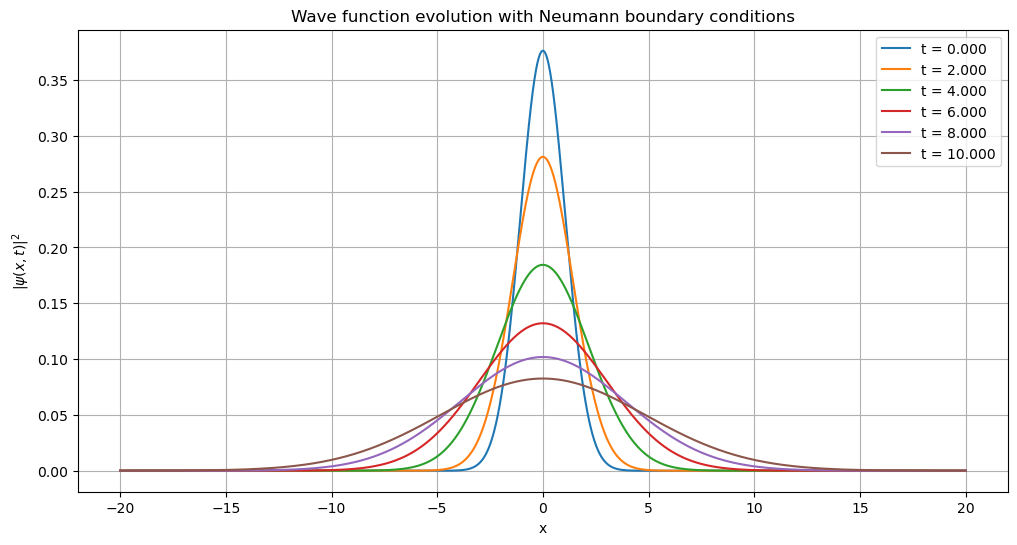
\includegraphics[width=\textwidth]{Immagini/plot-schrodinger-free-particle.png}
    \end{figure}
\end{frame}

\begin{frame}{Ballistic spreading}
    The numerical $\sigma$ follows the same \textbf{ballistic behaviour} up until the time when the wavefunction \underline{reaches the boundary}.

    \begin{equation*}
        \sigma(t)\propto\frac{t}{\sigma_0} \ \longrightarrow \ \text{Bigger $\sigma_0$, slower spreading}
    \end{equation*}

    \pause

    \vfill

    \visible<2>{\begin{minipage}{0.31\textwidth}
        \begin{center}
            $\sigma_0=0.10$
        \end{center}
        \vspace{-0.25cm}
        \begin{figure}
            \centering
            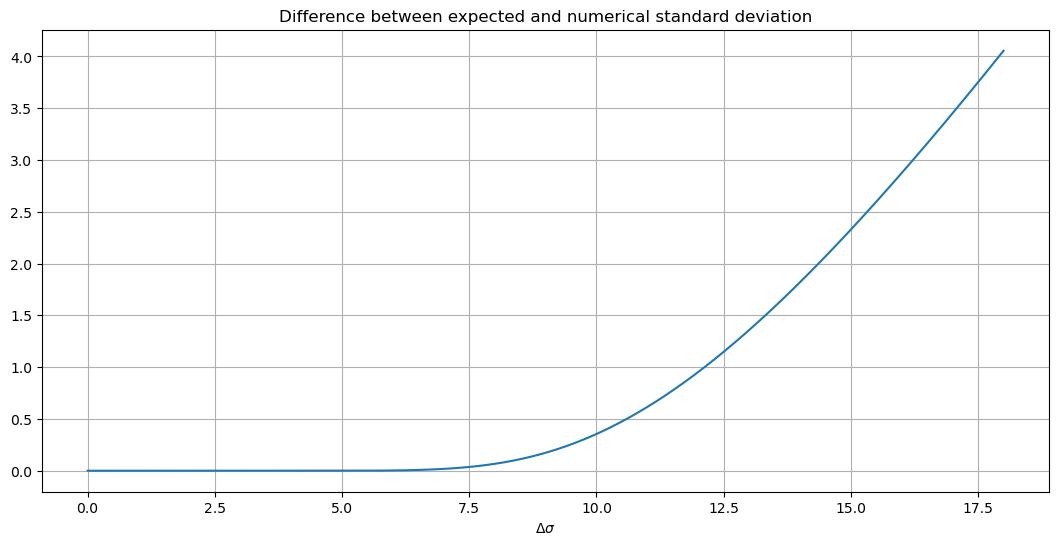
\includegraphics[width=\textwidth]{Immagini/plot-sigma-diff-1.png}
        \end{figure}
    \end{minipage}
    \hfill
    \begin{minipage}{0.31\textwidth}
        \begin{center}
            $\sigma_0=0.15$
        \end{center}
        \vspace{-0.25cm}
        \begin{figure}
            \centering
            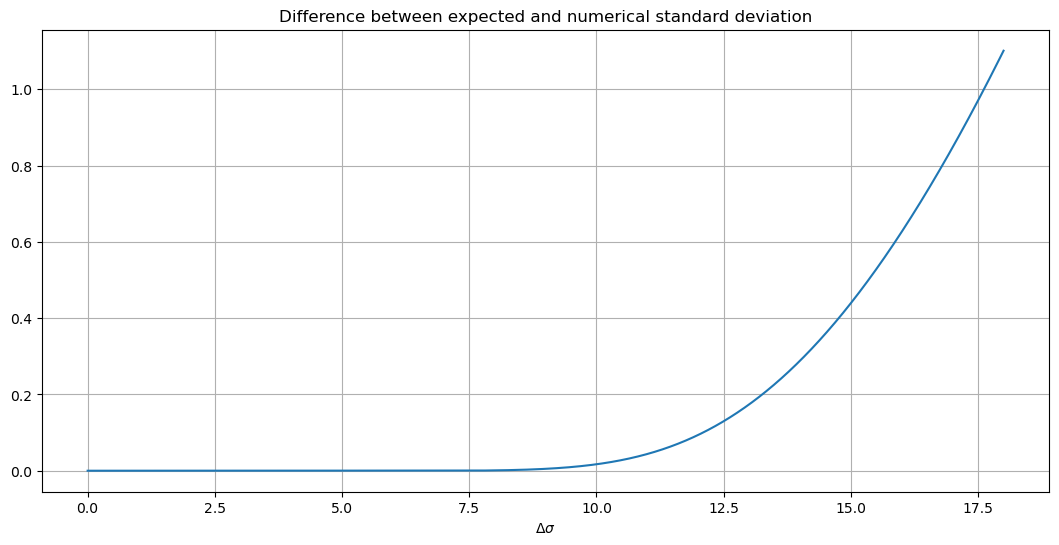
\includegraphics[width=\textwidth]{Immagini/plot-sigma-diff-1,5.png}
        \end{figure}
    \end{minipage}
    \hfill
    \begin{minipage}{0.31\textwidth}
        \begin{center}
            $\sigma_0=0.20$
        \end{center}
        \vspace{-0.25cm}
        \begin{figure}
            \centering
            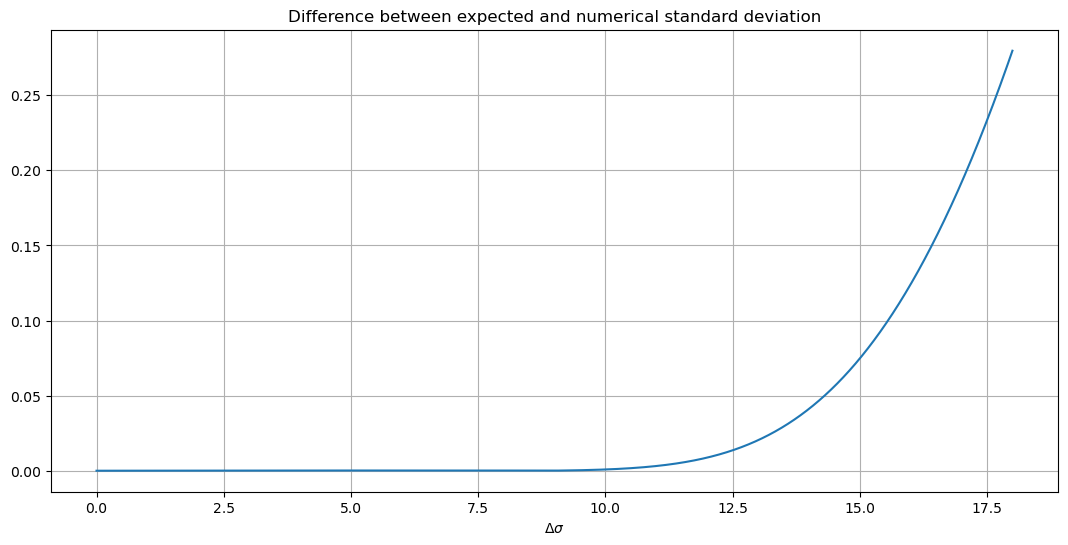
\includegraphics[width=\textwidth]{Immagini/plot-sigma-diff-2.png}
        \end{figure}
    \end{minipage}

    \vspace{-0.15cm}

    \begin{figure}[H]
        \centering
        \begin{tikzpicture}
            \draw[decorate, decoration={brace, amplitude=8pt, raise=2pt}] (5.45,0) -- (-5.45,0);

            \node at (0,-0.75) () {Smaller error with larger $\sigma_0$ at equal times};
        \end{tikzpicture}
    \end{figure}}
\end{frame}

\subsection{Periodic potential}

\begin{frame}{Kronig-Penney model}
    The introduction of a \textbf{periodic potential} leads to what is called a \textcolor{BrickRed}{\textbf{Kronig-Penney-like model}}, which is used to describe electrons in a \underline{crystal lattice}.

    \pause

    \begin{center}
      \begin{framed}
        \textcolor{BrickRed}{\textbf{Bloch's theorem}} states that solutions to the Schrödinger equation in a \underline{periodic potential} can be expressed as \textit{plane waves} modulated by \textit{periodic functions} $u(x)$ with the same periodicity as the crystal:

        \begin{equation*}
            \psi(x)=e^{ikx}u(x)
        \end{equation*}
      \end{framed}
   \end{center}
\end{frame}

\begin{frame}{Bloch waves}
    A periodic potential $V(x)=V_0\cos\left(\frac{2\pi}{a}x\right)$ couples plane waves which differ of multiples of $\frac{2\pi}{a}$, and the resulting superpositions form the \textcolor{BrickRed}{\textbf{Bloch waves}}.

    \vspace{-0.15cm}

    \begin{equation*}
        \text{Projection onto periodic plane waves}
    \end{equation*}

    \vspace{-0.3cm}

    \begin{equation*}
        \Big\downarrow
    \end{equation*}

    \vspace{-0.25cm}

    \begin{equation*}
        \text{Formation of \textbf{lattice harmonics}}
    \end{equation*}

    \vfill

    \begin{minipage}{0.32\textwidth}
        \begin{center}
            $a=1.0$
        \end{center}
        \vspace{-0.25cm}
        \begin{figure}
            \centering
            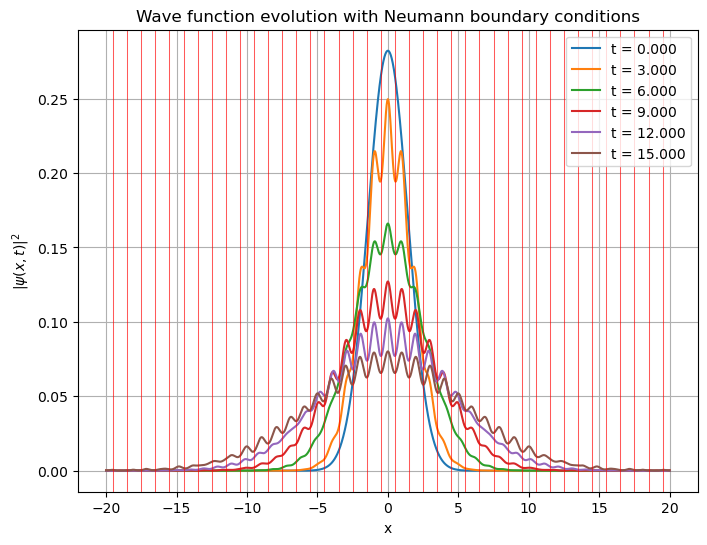
\includegraphics[width=\textwidth]{Immagini/plot-periodic-potential-a-1.png}
        \end{figure}
    \end{minipage}
    \hfill
    \begin{minipage}{0.32\textwidth}
        \begin{center}
            $a=1.5$
        \end{center}
        \vspace{-0.25cm}
        \begin{figure}
            \centering
            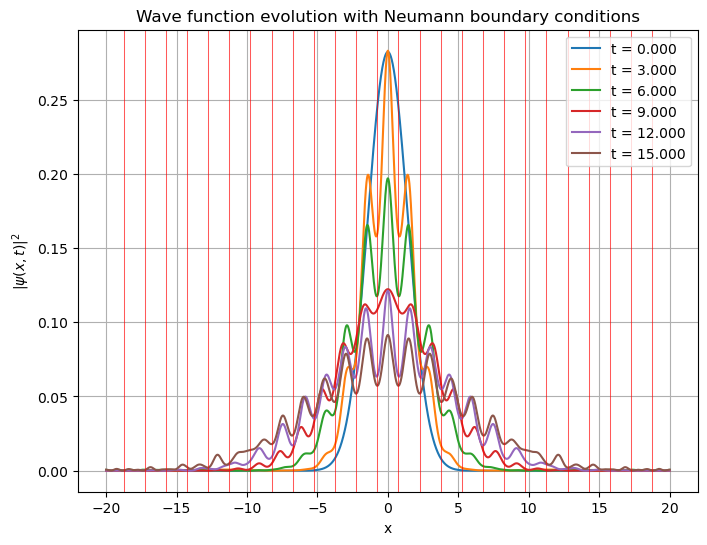
\includegraphics[width=\textwidth]{Immagini/plot-periodic-potential-a-1,5.png}
        \end{figure}
    \end{minipage}
    \hfill
    \begin{minipage}{0.32\textwidth}
        \begin{center}
            $a=2.0$
        \end{center}
        \vspace{-0.25cm}
        \begin{figure}
            \centering
            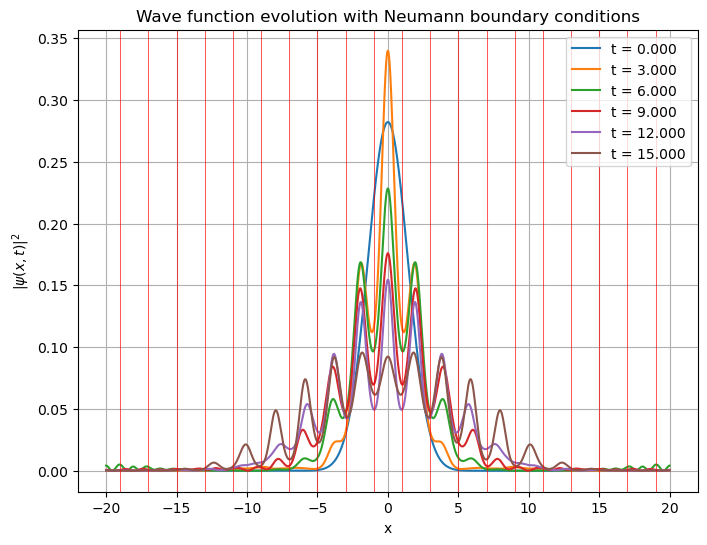
\includegraphics[width=\textwidth]{Immagini/plot-periodic-potential-a-2.png}
        \end{figure}
    \end{minipage}
\end{frame}

\begin{frame}{Effective mass}
    \small

    With the periodic potential, the allowed energies are \underline{no longer continuous}, but split into separate \textbf{bands}, each associated with different values of the \textit{crystal momentum} $k$.

    \vfill

    \pause

    \footnotesize

    Taylor expansion around $k_0$:

    \begin{equation*}
        E(k)=E\left(k_0\right)+\frac{dE}{dk}\bigg|_{k_0}\left(k-k_0\right)+\frac{1}{2}\frac{d^2E}{dk^2}\bigg|_{k_0}\left(k-k_0\right)^2+\dots
    \end{equation*}

    \pause

    In the lowest bound, $k_0=0$ is the \textit{minimum}:

    \begin{equation*}
        E(k)\simeq E_0+\frac{1}{2}\frac{d^2E}{dk^2}\bigg|_{k=0}k^2
    \end{equation*}

    \pause

    Comparing with the energy of a free particle, an \textcolor{BrickRed}{\textbf{effective mass}} can be found:

    \begin{equation*}
        E(k)=E_0+\frac{\hbar^2k^2}{2m^*} \ \Longrightarrow \ \fcolorbox{BrickRed}{white}{\text{$\displaystyle m^*=\hbar^2\left(\frac{d^2E}{dk^2}\bigg|_{k=0}\right)^{-1}$}}
    \end{equation*}

    \normalsize
\end{frame}

\begin{frame}{Sub-ballistic spreading}
    \small

    Around the \textit{minimum of a band}, a quantum system in a periodic lattice behaves like a free particle with an effective mass $m^*$.

    \vfill

    Since $\sigma\propto\frac{1}{m}$, a slower spreading is expected for a periodic lattice where $m^*>m$, due to the \textbf{parabolic approximation} of the band energy.

    \vfill

    \begin{figure}[H]
        \centering
        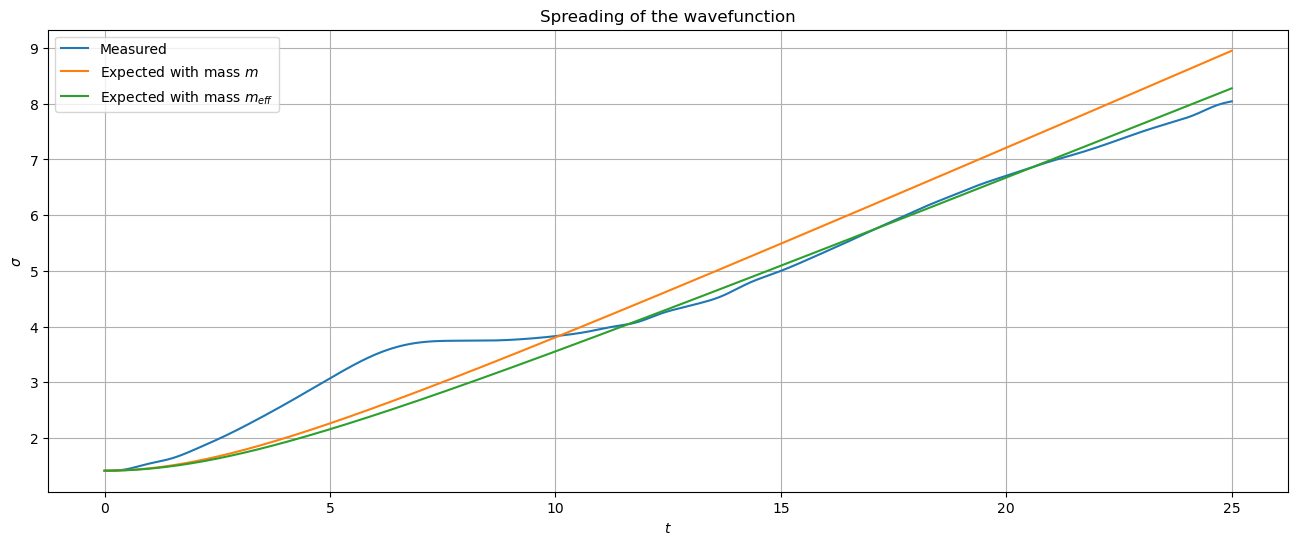
\includegraphics[width=\textwidth]{Immagini/plot-effective-mass.png}
    \end{figure}

    \normalsize
\end{frame}

\subsection{Linear potential}

\begin{frame}{Addition of a linear term}
    The mean value, on the contrary, \underline{does not change}.

    \vfill

    \pause

    In order to induce a \textit{net drift}, we must add a \textbf{linear potential} $V(x)=Fx$.

    \vfill

    \vspace{-0.1cm}

    \visible<2>{\begin{figure}[H]
        \centering
        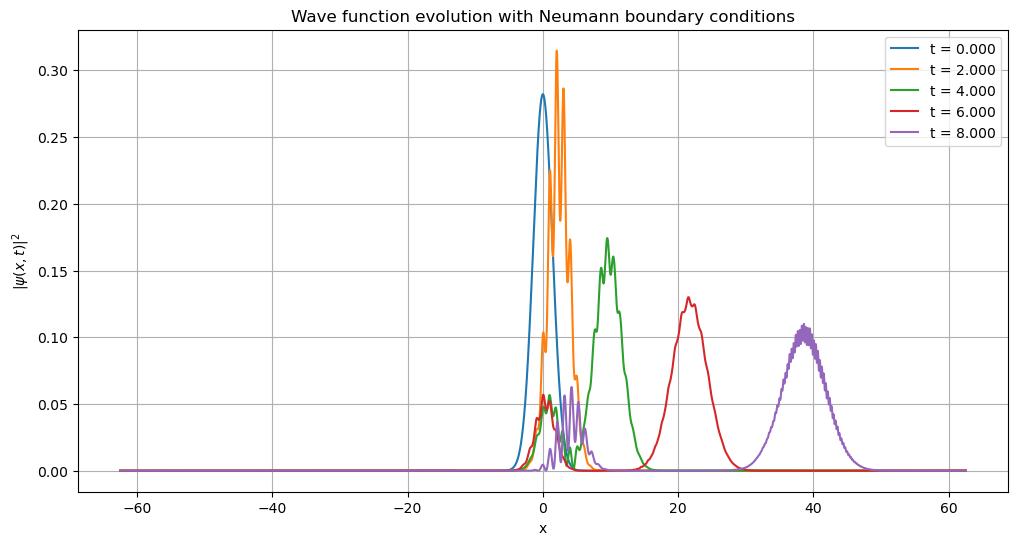
\includegraphics[width=0.87\textwidth]{Immagini/plot-linear-potential.png}
    \end{figure}}

    \vspace{-0.5cm}

    \footnotesize

    \begin{center}
        The plot shows how \underline{dispersion} causes \textbf{interference effects} to gradually \textit{fade}.
    \end{center}

    \normalsize
\end{frame}

\begin{frame}{Average shift}
    \vfill

    \begin{minipage}[c]{0.45\textwidth}
        \begin{figure}
            \centering
            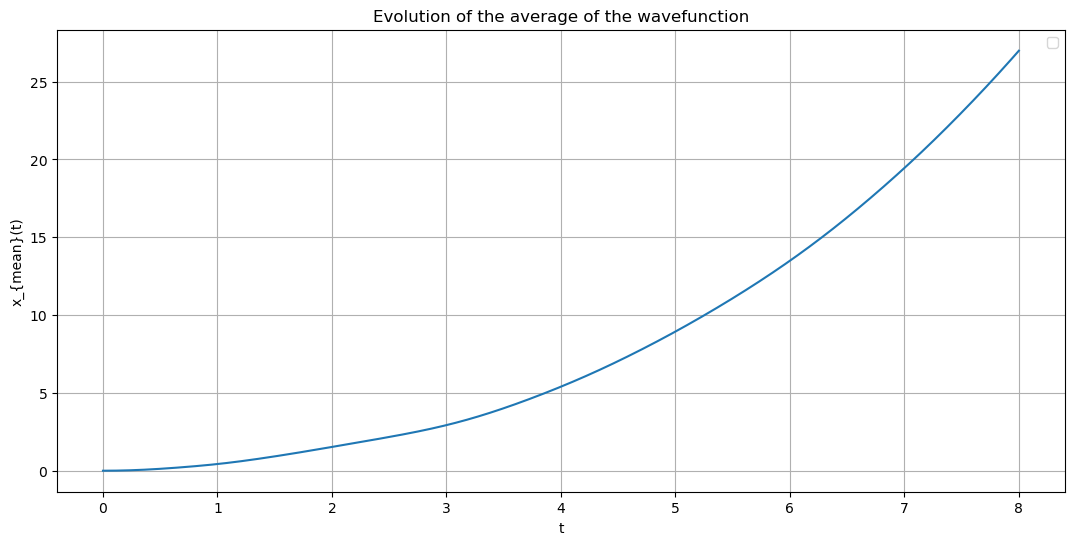
\includegraphics[width=\textwidth]{Immagini/plot-moving-average-1.png}
            \caption*{$V_0=1.00$, $F=1.00$}
        \end{figure}
    \end{minipage}
    \hfill
    \begin{minipage}[c]{0.45\textwidth}
        \begin{figure}
            \centering
            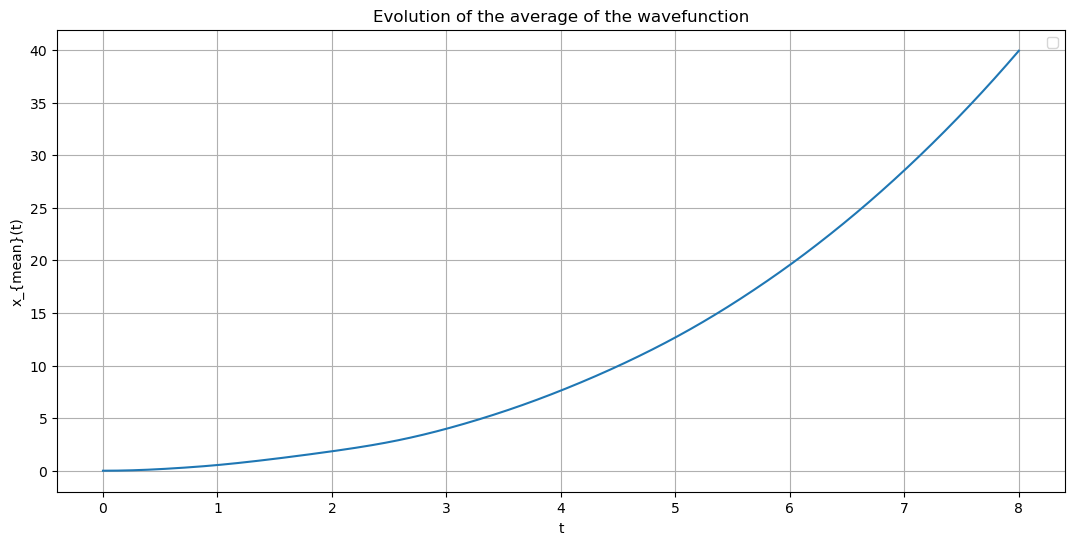
\includegraphics[width=\textwidth]{Immagini/plot-moving-average-1,25.png}
            \caption*{$V_0=1.00$, $F=1.25$}
        \end{figure}
    \end{minipage}

    \vfill

    \begin{minipage}[c]{0.45\textwidth}
        \begin{figure}
            \centering
            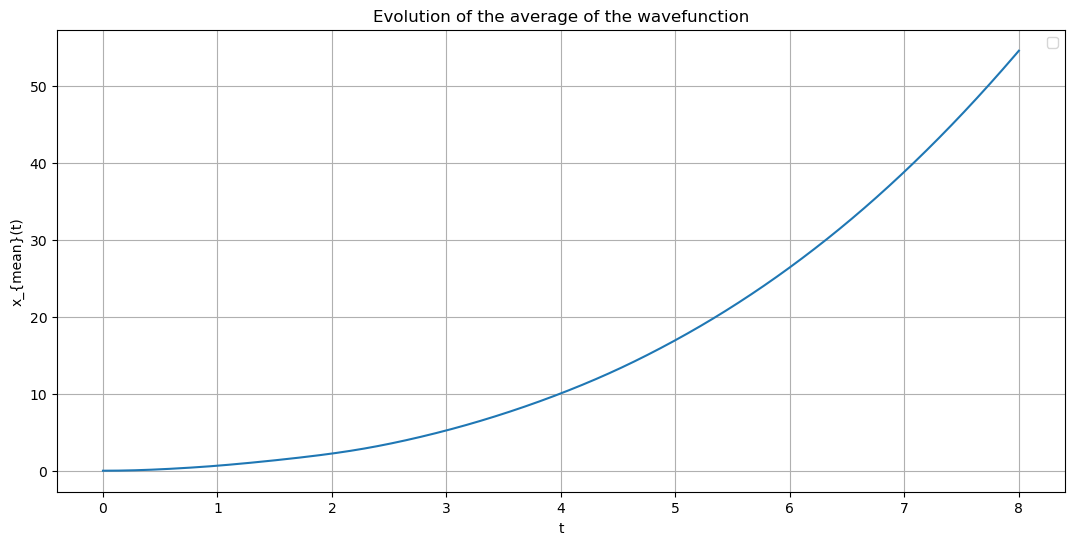
\includegraphics[width=\textwidth]{Immagini/plot-moving-average-1,5.png}
            \caption*{$V_0=1.00$, $F=1.50$}
        \end{figure}
    \end{minipage}
    \hfill
    \begin{minipage}[c]{0.45\textwidth}
        \begin{figure}
            \centering
            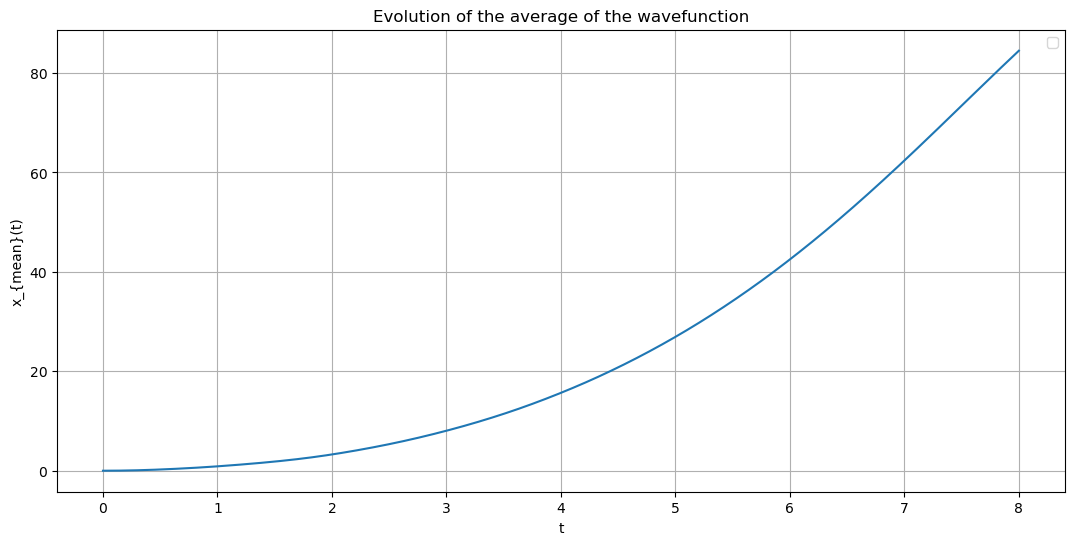
\includegraphics[width=\textwidth]{Immagini/plot-moving-average-2.png}
            \caption*{$V_0=1.00$, $F=2.00$}
        \end{figure}
    \end{minipage}
\end{frame}

\begin{frame}{Conclusions}
    Some final considerations:

    \vfill

    \pause

    \begin{itemize}
        \item FEM provides a suitable approach for \textbf{second-order PDEs}
        \pause
        \item Even though it has been used for very simple domains, in principle it can be applied to very \textbf{complex geometries}
        \pause
        \item To handle time evolution, FEM must be coupled with \textbf{finite difference schemes} or other temporal integration methods
        \pause
        \item The choice of spatial mesh and time step must satisfy some \textbf{stability} and \textbf{accuracy criteria} (like CFL condition or norm conservation)
        \pause
        \item FEM allows easy incorporation of \textbf{boundary conditions}
    \end{itemize}

    \vfill

    \pause

    In summary, our examples show that FEM is a very \textbf{robust} and \textbf{versatile} tool for \underline{spatial discretization}, but time evolution requires \textit{appropriate temporal schemes}.
\end{frame}

\end{document}